%% ============================================================
%% Governance Constellations in Innovation Ecosystems:
%% A Computational Role Analysis of EIT Co-creation Networks
%%
%% Submitted to Environmental Innovation and Societal Transitions
%% Special Issue: "Stimulating Local Co-creation for Transformative Change"
%%
%% Deadline: April 2026
%% ============================================================

\documentclass[review,12pt]{elsarticle}

%% --- Packages ---
\usepackage[T1]{fontenc}
\usepackage[utf8]{inputenc}
\usepackage{lmodern}
\usepackage{microtype}
\usepackage{booktabs}
\usepackage{array}
\usepackage{longtable}
\usepackage{tabularx}
\usepackage{multirow}
\usepackage{graphicx}
\usepackage{float}
\usepackage{caption}
\usepackage{amsmath}
\usepackage{amssymb}
\usepackage{xcolor}
\usepackage{hyperref}
\hypersetup{
  colorlinks=true,
  linkcolor=black,
  citecolor=black,
  urlcolor=black,
  pdfborder={0 0 0}
}
\usepackage{enumitem}
\usepackage{tikz}
\usetikzlibrary{shapes.geometric,arrows.meta,positioning,fit,backgrounds,calc}
\usepackage{pgfplots}
\pgfplotsset{compat=1.18}

%% --- Bibliography (natbib for EIST) ---
\biboptions{round,authoryear,sort&compress}
\bibliographystyle{elsarticle-harv}

%% Line spacing for review (double-spaced)
\usepackage{setspace}
\doublespacing

%% Paragraph spacing
\setlength{\parskip}{0.5em}
\setlength{\parindent}{1.5em}

%% Line numbering for review
\usepackage{lineno}
\modulolinenumbers[5]

%% Possessive citation form: \citepos{key} -> Author's (year)
\newcommand{\citepos}[1]{\citeauthor{#1}'s \citeyearpar{#1}}

%% --- Custom colors for actor types ---
\definecolor{CityBlue}{RGB}{31,119,180}
\definecolor{UniViolet}{RGB}{148,103,189}
\definecolor{CompGreen}{RGB}{44,160,44}
\definecolor{NGOAmber}{RGB}{255,165,0}
\definecolor{KICRed}{RGB}{214,39,40}
\definecolor{HubRed}{RGB}{214,39,40}
\definecolor{BridgeOrange}{RGB}{255,127,14}
\definecolor{AmpTeal}{RGB}{44,160,44}
\definecolor{RecBlue}{RGB}{31,119,180}
\definecolor{KTEdu}{RGB}{70,130,180}
\definecolor{KTRes}{RGB}{34,139,34}
\definecolor{KTBus}{RGB}{178,34,34}
\definecolor{PipeGray}{RGB}{100,100,100}

%% ============================================================
\begin{document}

\begin{frontmatter}

\title{Governance Constellations in Innovation Ecosystems: A Computational Role Analysis of EIT Co-creation Networks}

\author[rsm]{Babajide Owoyele}
\address[rsm]{Rotterdam School of Management, Erasmus University, Burgemeester Oudlaan 50, 3062 PA Rotterdam, The Netherlands}
\ead{b.owoyele@rsm.nl}

\begin{abstract}
Co-creation governance research has identified a persistent gap: despite their central role in urban climate transition, cities remain structurally peripheral in European innovation ecosystems. This paper operationalizes Ansell and Torfing's (2021) ``governance constellation'' concept through a computational role analysis of 219 actors participating in the European Institute of Innovation and Technology (EIT) co-creation network, comprising 111 NetZeroCities municipal partners and 108 EIT Knowledge and Innovation Community (KIC) organizations. We apply RoleSim, a network role classification method, to two data layers --- Wikipedia text-similarity networks and Twitter co-mention graphs (268,000 tweets; 500 actors) --- to assign each actor one of four structural roles: Hub, Bridge, Amplifier, or Receiver. Results reveal that 72\% of cities occupy Receiver positions and only 6\% serve as Hubs, exposing a structural asymmetry that impedes city-led co-creation. Hub density at the KIC level correlates strongly with co-creation output: EIT InnoEnergy (16.9\% Hub density) achieves 82\% venture funding rates versus EIT Urban Mobility (1.7\% Hub density) at 56.9\%. Ten Bridge actors function as cross-KIC governance infrastructure. Knowledge Triangle analysis shows cities averaging KT\_Business = 0.41, lower than KIC hubs (KT\_Business = 0.62), indicating misaligned incentive architectures. Governance simulation experiments suggest that strategically elevating 15 cities to Hub-adjacent roles would increase predicted co-creation output by approximately 23\%. We conclude by proposing a typology of governance constellations --- Hub-dense, Bridge-dependent, and Receiver-heavy --- with distinct reform implications for EIT and NetZeroCities programme design.
\end{abstract}

\begin{keyword}
co-creation \sep governance constellations \sep innovation ecosystems \sep network role analysis \sep knowledge triangle \sep EIT \sep NetZeroCities \sep sustainability transitions
\end{keyword}

\begin{highlights}
\item Cities occupy Receiver roles in 72\% of cases, revealing structural barriers to city-led co-creation in EIT networks.
\item KIC Hub density predicts co-creation output: 16.9\% Hub density (InnoEnergy) yields 82\% funded ventures versus 56.9\% for low-Hub KICs.
\item Ten Bridge actors serve as cross-KIC connectors, constituting the governance infrastructure of the ecosystem.
\item Knowledge Triangle profiling reveals cities' business-sector orientation (KT\_Business = 0.41) lags KIC hubs (0.62), indicating incentive misalignment.
\item Governance simulation demonstrates that targeted role redistribution can increase co-creation output by approximately 23\%.
\end{highlights}

\end{frontmatter}

%% ============================================================
\section{Introduction}
\label{sec:intro}
%% ============================================================

Urban climate transitions cannot be accomplished by central governments alone. They require what \citet{ansell2021co} term co-creation: the collaborative development and implementation of novel solutions in which public, private, and civic actors pool resources, knowledge, and legitimacy across institutional boundaries. The climate emergency has transformed this theoretical aspiration into a practical urgency: the European Union's Fit for 55 legislative package and its Mission on 100 Climate-Neutral and Smart Cities have set legally binding decarbonisation targets that no single actor class can achieve in isolation \citep{european2021fit, mazzucato2018mission}. Cities, which account for over 70\% of global energy consumption and carbon emissions, are simultaneously the primary sites of climate impact and the primary arenas in which transformative co-creation must occur \citep{bulkeley2013urban}.

Yet despite rhetorical commitments to co-creation embedded in flagship European programmes --- from the European Green Deal to the NetZeroCities Pilot Cities Programme --- systematic evidence on how governance structures enable or constrain local actors' participation in co-creation processes remains sparse \citep{holscher2018navigating, sorensen2017metagovernance}. The co-creation literature has developed rich conceptual frameworks and qualitative case studies, but lacks computational methods capable of characterising governance arrangements across the hundreds of actors that constitute a real innovation ecosystem \citep{grimmer2021machine}. This methodological gap has practical consequences: governance reforms targeting co-creation are designed without a structural understanding of the arrangements they aim to change.

The European Institute of Innovation and Technology (EIT) constitutes the largest organised co-creation infrastructure in Europe. Established by the European Commission in 2008, it now coordinates nine Knowledge and Innovation Communities (KICs) spanning climate, energy, food, health, manufacturing, raw materials, digital innovation, urban mobility, and cultural and creative industries. Across these KICs, the EIT coordinates over 600 partner organisations comprising universities, research centres, companies, and public bodies, with an annual budget exceeding €500 million. The programme's co-creation mandate is embedded in its founding regulation: KICs must demonstrate integration across the Knowledge Triangle of Education, Research, and Business --- the Triple Helix of institutional collaboration that \citet{etzkowitz2000dynamics} identified as the generative mechanism of knowledge-economy innovation.

The NetZeroCities (NZC) programme extends this architecture to urban climate governance, enlisting 111 European municipalities as pilot cities in a shared commitment to carbon neutrality by 2030, co-created alongside EIT partners \citep{nzc2022pilot}. NZC represents an explicit institutionalisation of the co-creation agenda: cities are not merely target beneficiaries of EIT solutions but designated co-creators, formally enrolled in governance structures designed to generate locally adapted climate innovations. Whether this architecture delivers on its co-creation promise --- or reproduces the structural asymmetries that have historically sidelined cities from agenda-setting in European innovation policy --- is an open and consequential empirical question.

This paper addresses that question through a computational analysis of governance structure. Our central contribution is methodological and substantive: we operationalise \citepos{ansell2021co} ``governance constellation'' concept --- the configuration of actor types, relational ties, and institutional rules that enable or suppress co-creation --- using RoleSim \citep{owoyele2024rolesim}, a network role classification algorithm that identifies structural positions (Hub, Bridge, Amplifier, Receiver) from multi-source network data. By applying RoleSim to a 219-actor network constructed from Wikipedia text-similarity graphs, Twitter co-mention networks, and encyclopaedic co-citation data, we produce the first large-scale empirical map of governance constellations in the EIT co-creation system. This approach implements the data science research cycle described by \citet{maass2018data} --- Curation, Annotation, Unsupervised Analysis, Output --- in a governance analysis context, demonstrating how computational IS methods can bridge the gap between co-creation as discursive aspiration and co-creation as structural reality.

Our findings reveal a striking structural asymmetry that calls into question the co-creation characterisation of the EIT-NetZeroCities architecture. Cities are predominantly Receivers in the EIT network, positioned to absorb expertise and funding rather than to generate agendas or broker connections: 72\% of the 111 NZC pilot cities occupy Receiver roles, and only 6\% function as Hubs. This contrasts sharply with KIC organisational units, 31\% of which are classified as Hubs. The architecture is not neutral with respect to co-creation outcomes: Hub density at the KIC level correlates with venture funding rates at $r = 0.94$ ($p < 0.001$), and cities' structural peripherality corresponds to a 21-percentage-point gap in Knowledge Triangle Business scores relative to KIC hubs ($0.41$ vs.\ $0.62$), indicating that the incentive structures embedded in the EIT's commercialisation metrics systematically reproduce urban marginalisation.

These findings speak directly to the central concern of this Special Issue: what constellations of governance factors enable transformative co-creation? We demonstrate that role structure --- the distribution of Hub, Bridge, Amplifier, and Receiver positions across actor types --- is the proximate governance factor distinguishing effective from ineffective co-creation ecosystems. Diversity of actor types, as embodied in the EIT's cross-sector partnership model, is a necessary but not sufficient condition; structural role distribution determines whether that diversity translates into genuine co-creative agency or merely into a more diverse population of Receivers. Our governance simulation analyses show that targeted structural interventions --- elevating 15 strategically positioned cities from Receiver to Hub-adjacent roles, seeding new Bridge actors --- could increase projected co-creation output by over 22--31\%, providing an evidence base for EIT governance reform that goes beyond rhetorical reaffirmation of the co-creation mandate.

The paper proceeds as follows. Section~\ref{sec:theory} develops the theoretical framework, integrating governance constellation theory, Knowledge Triangle models, and computational ecosystem methodology. Section~\ref{sec:design} presents the research design and the nine-step Basole framework as adapted for governance analysis. Section~\ref{sec:data} details data sources and network construction. Section~\ref{sec:results} presents role analysis findings. Section~\ref{sec:simulation} reports governance simulation experiments. Section~\ref{sec:discussion} discusses implications for theory and EIT reform. Section~\ref{sec:conclusion} concludes.

%% ============================================================
\section{Theoretical Background}
\label{sec:theory}
%% ============================================================

\subsection{Co-creation Governance: From Participation to Constellations}

Co-creation as a governance concept has developed through several generations of scholarship, each advancing the analytical precision with which participation, power, and structural arrangement are theorised. The foundational work on co-production established that citizens and service users could contribute substantively to the delivery of public services --- contributing labour, knowledge, contextual information, or local social capital that supplement and sometimes surpass what state actors can provide alone \citep{ostrom1996crossing, bovaird2007beyond}. Systematic reviews of this literature established that co-production yields better-adapted outputs, increases user legitimacy, and builds social capital across the citizen-state relationship \citep{voorberg2015systematic}. However, early co-production theory left underspecified the governance conditions that distinguish meaningful co-production from token consultation, and the relational architectures that determine which actors can effectively participate.

\citet{ansell2008collaborative} advanced the analysis through their collaborative governance framework, drawing on a systematic review of cases to identify six variables that modulate participation quality: the history of prior conflict or cooperation among actors, incentive structures for participation, power asymmetries in resource endowment and agenda-setting, leadership quality, institutional design of the collaborative forum, and the iterative dynamics of the collaborative process itself. This framework has been widely applied to governance analysis in sustainability, urban policy, and public service reform contexts. What it lacked, however, was an explicitly structural dimension: the Ansell-Gash model treats governance as a set of enabling or constraining conditions experienced by participating actors, rather than as a configuration --- a relational arrangement of positions and flows that enables or forecloses specific actor behaviours irrespective of individual actors' capacities or intentions.

\citet{ansell2021co} provided this structural corrective through the concept of governance constellations. Their argument is that co-creation is not a dyadic relationship between a public authority and a partner organisation, but a systemic property emerging from the configuration of multiple actors, each occupying distinct positions in a relational field that is irreducible to the sum of its bilateral ties. A governance constellation is characterised by its \emph{density} --- how many actors occupy hub-like, agenda-setting roles from which they can define co-creation problems and criteria --- its \emph{architecture} --- whether power and information flow through distributed bridges or concentrate in a small core of dominant actors --- and its \emph{coherence} --- whether different actor types share sufficiently compatible incentive structures to sustain collective action across institutional boundaries. Constellations can be more or less enabling of transformative co-creation independently of the formal mandates, stated intentions, or individual capacities of participating organisations.

This conceptual advance creates an immediate operationalisation problem. Governance constellations are relational and multi-level, emergent from the aggregate pattern of ties across a population of actors; yet most governance research collects data on individual actors or bilateral relationships, and administrative records rarely capture the informal network structure that gives a constellation its co-creative character. \citet{torfing2019co} acknowledge this gap, noting that measuring constellations requires network data that is typically unavailable in programme documentation or survey responses. The absence of appropriate measurement methods has prevented governance constellation theory from moving from normative prescription to empirical diagnosis. Computational methods offer a path forward.

\subsection{Untapped Co-creation Potential and the X-Curve Problem}

The sustainability transitions literature has independently developed arguments about structural barriers to co-creative governance that complement and deepen the governance constellation framework. \citet{hebinck2023untapped} use the X-curve framework --- which models sustainability transitions as the simultaneous decline of incumbent unsustainable systems and the growth of sustainable alternatives --- to argue that cities and urban actors possess substantial \emph{untapped} co-creation potential: the knowledge, legitimacy, and territorial embeddedness that would make them essential partners in transition, but which the governance structures of dominant innovation systems fail to mobilise.

The X-curve diagnosis maps directly onto our empirical findings: the EIT ecosystem's co-creation rhetoric represents the ascending arm of ambition, while the structural Receiver pattern among cities represents the stalled growth of city-led co-creation that this ambition has not yet unlocked. \citet{loorbach2017sustainability} similarly identify power asymmetries between incumbent regime actors (large universities, multinational companies, public research institutes) and transition-oriented niche actors (municipalities, community organisations, social enterprises) as a central mechanism sustaining unsustainable path dependencies. In the EIT context, KIC hub organisations and well-connected research universities function as incumbent regime actors in the innovation governance sense: they occupy Hub and Bridge roles that allow them to define co-creation agendas, select partners, and determine what counts as a co-creation success, while cities remain in peripheral Receiver positions regardless of their climate ambition or governance capacity.

\citet{coenen2012place} extend this critique with a spatial argument: sustainability transitions research has systematically under-valued the place-specific, politically embedded dimensions of transition governance, focusing on sectoral and technological dynamics while treating the places where transitions must ultimately materialise as passive implementation sites. The EIT ecosystem instantiates precisely the dynamic Coenen et al. critique: cities are the places where European urban climate transitions must occur, and they are formally enrolled in co-creation structures, yet their structural position as Receivers means that the content and direction of that co-creation is determined by actors operating at a spatial and institutional remove from urban realities.

\subsection{The Knowledge Triangle as an Incentive Architecture}

The Knowledge Triangle (KT) --- the conceptual space defined by Education (E), Research (R), and Business (B) axes --- was developed within the Triple Helix tradition to characterise actor types in innovation systems by their primary knowledge-exchange orientation \citep{etzkowitz2000dynamics, ranga2013triple}. The Triple Helix model posits that innovation in knowledge economies emerges from the productive interpenetration of university, industry, and government spheres, with each sphere contributing distinctive resources: universities contribute knowledge creation and human capital development; industry contributes market access and applied innovation capacity; government contributes regulatory frameworks, public procurement power, and legitimating authority. The KT operationalises this three-sphere model by positioning each actor type as oriented primarily toward one of three knowledge functions: Education (training human capital), Research (generating codified knowledge), or Business (translating knowledge into market value).

The EIT was explicitly designed around the KT: each KIC is required to demonstrate cross-sector partnerships spanning all three axes, with governance boards typically including academic, corporate, and public-sector representatives. Annual KIC performance metrics include the EIT Label for higher education programmes (measuring Education axis contribution), publication and patent counts (measuring Research axis contribution), and venture creation and revenue generation metrics (measuring Business axis contribution). The KT thus functions simultaneously as a formal governance rule determining who must be present in KIC governance and as an implicit theory of complementarity specifying what different actor types are expected to contribute.

What the KT framework has not systematically addressed, however, is whether the formal presence of diverse actor types translates into equivalent co-creation capacity, or whether actors with nominally similar KT profiles but different structural positions perform very different governance functions. A city with KT\_Business = 0.41 and KT\_Research = 0.28 may be formally present in an EIT governance body alongside a KIC hub with KT\_Business = 0.62, yet the structural positions they occupy --- and therefore the co-creative roles they can effectively perform --- differ dramatically. The city's business orientation reflects public procurement and local economic development functions; the KIC hub's business orientation reflects technology commercialisation and venture investment. These are institutionally distinct orientations that the KT scalar score conflates. KT profiling is thus necessary but not sufficient for characterising co-creation capacity; it must be complemented by structural role analysis that distinguishes position from profile.

A deeper theoretical grounding for the Knowledge Triangle is provided by \citet{oberg2017culture} and \citet{korff2015interstitial}, who conceptualise innovation fields as simultaneously relational structures and meaning systems organised around three institutional logics: Associational (shared identity and civic purpose), Scientific (epistemic authority and knowledge validation), and Managerial (market efficiency and value capture). These three logics map directly onto the EIT Knowledge Triangle's three axes: Education corresponds to the Associational logic through which universities and public bodies build shared professional communities; Research corresponds to the Scientific logic that governs epistemic legitimacy and publication norms; Business corresponds to the Managerial logic that drives commercialisation and venture formation. The KT is not, therefore, a neutral measurement instrument --- it encodes a particular configuration of institutional logics whose relative weight in any given ecosystem determines which actors are recognised as legitimate co-creators. \citet{powell1996interorganizational}'s foundational finding that triadic embeddedness across firm, university, and research institute --- the organisational instantiation of all three KT vertices simultaneously --- predicts innovation output in knowledge-intensive sectors reinforces this interpretation: the KT triangle is itself a theory of structural complementarity, and actors who span all three logics occupy the governance positions best suited to convening, brokering, and amplifying co-creation across the ecosystem.

\subsection{Computational Innovation Ecosystem Analysis}

The ecosystem metaphor has productively reoriented innovation studies from linear models of knowledge transfer to systemic models of co-evolutionary value creation among diverse, interdependent actors \citep{jacobides2018towards}. Innovation ecosystems are characterised by modularity, role differentiation, and the emergence of distinct structural specialisations: platform organisations that coordinate complementors, integrators that bundle modular components, and user-innovators who both consume and contribute to the ecosystem's knowledge base \citep{fagerberg2005innovation}. The governance challenge for co-creation in innovation ecosystems is to design architectures in which this role differentiation is productive rather than exclusionary --- in which the structural positions of different actor types reflect their genuine comparative advantages rather than historical path dependencies or institutional power imbalances.

\citet{basole2023computational} operationalised innovation ecosystem analysis as a nine-step computational methodology that moves from data curation through network construction, metric computation, interactive visualisation, structured sensemaking, hypothesis generation, scenario construction, simulation, and design recommendation. This framework has been applied to startup ecosystems, enterprise platform networks, and inter-firm R\&D collaboration networks. Its key contribution is treating ecosystem analysis as a design science activity \citep{hevner2004design}: not merely mapping what exists, but generating actionable knowledge about what could exist under alternative design choices, and providing a replicable, transparent methodology for doing so. Within this framework, entropy functions as a diagnostic dimension of ecosystem health: actors with low behavioural entropy exhibit rule-abiding, stable participation patterns --- their relational repertoire is predictable and institutionally constrained --- while actors with high behavioural entropy exhibit rule-changing, exploratory behaviour that is characteristic of transitional or niche-level agency \citep{basole2023computational}. Governance constellation analysis extends this insight by linking entropy to structural role: Receiver actors tend toward low entropy because the absorptive logic of their position constrains the variety of relational moves available to them, whereas Hub and Bridge actors tend toward higher entropy because their agenda-setting and brokering functions require them to generate novel connections across institutional domains.

For governance constellation analysis, the computational turn offers three specific advantages beyond qualitative methods. First, multi-source data integration --- combining text-based semantic similarity networks with social media co-mention graphs and bibliometric co-citation networks --- captures governance relationships that do not appear in formal organisational charts or partnership registries but are nonetheless consequential for co-creation dynamics. Informal influence, repeated public co-endorsement, and encyclopaedic proximity are all governance-relevant relationships that only digital trace data can reveal at scale. Second, role classification through network metrics provides a systematic, replicable operationalisation of structural position that removes the interpretation ambiguity inherent in qualitative typologies; the same algorithm applied to different time points or different ecosystems produces comparable role assignments. Third, simulation experiments enable counterfactual governance analysis: holding network topology constant while varying role distributions allows us to estimate the structural consequences of governance reforms before they are implemented, generating evidence-based policy guidance.

\subsection{RoleSim as Governance Constellation Operationalization}

RoleSim is a network role classification algorithm specifically designed for multi-actor innovation ecosystems \citep{owoyele2024rolesim}. It assigns each actor to one of four primary roles by computing a four-dimensional centrality profile --- degree, eigenvector centrality, betweenness centrality, and in/out-degree asymmetry --- and classifying actors into role clusters through an unsupervised $k$-means procedure ($k = 4$) validated through silhouette analysis and theoretical coherence review. The four roles correspond to distinct structural and governance functions:

\textbf{Hubs} are actors with high eigenvector centrality and high overall degree, connected to many well-connected others in a mutually reinforcing pattern. Their removal would substantially fragment the network by eliminating the dense tie concentrations that give the ecosystem its navigability. In governance terms, Hubs are agenda-setters and conveners: organisations whose participation is essential for others to coordinate around shared problems and priorities. Hub status reflects accumulated relational capital that enables simultaneous connection to multiple actor clusters.

\textbf{Bridges} are actors with high betweenness centrality relative to their degree: they occupy structurally sparse positions but lie on many of the shortest paths between otherwise disconnected clusters, functioning as essential conduits for information, resources, and legitimacy to flow across community boundaries. In governance terms, Bridges are boundary spanners \citep{howells2006intermediation}: organisations that translate across sectoral, institutional, or disciplinary divides, preventing the ecosystem from fragmenting into isolated and mutually ignorant sub-networks.

\textbf{Amplifiers} are actors with high out-degree relative to in-degree: they generate more outgoing connections than they receive, disseminating information, resources, and endorsements across the ecosystem more than they absorb them. In governance terms, Amplifiers are mobilisers: organisations that scale innovations, propagate knowledge, and expand the reach of Hub-generated agendas to actors who might otherwise remain outside the co-creation conversation.

\textbf{Receivers} are actors with high in-degree relative to out-degree: they attract substantial attention, resources, and information from the wider network but generate relatively few outgoing connections. In governance terms, Receivers are implementers and adopters: organisations that absorb and apply solutions developed elsewhere, contributing contextual knowledge and local legitimacy to implementation but playing a limited role in agenda-setting or knowledge brokering.

This role taxonomy maps directly onto the governance constellation dimensions identified by \citet{ansell2021co}. Hub density operationalises distributed co-creative leadership; Bridge count operationalises cross-sectoral integration capacity; the Amplifier-to-Receiver ratio operationalises the directionality of knowledge and resource flows --- whether the ecosystem generates and diffuses innovation upward and outward from peripheral actors, or funnels resources downward from a small core. Together, these metrics transform governance constellation theory from a normative typology into an empirically measurable network property, enabling systematic comparison across KICs, actor types, and time periods.

The connection to sustainability transitions theory is direct and consequential. \citet{schot2018three} argue that transformative innovation policy --- their third frame, beyond the R\&D support frame and the systems of innovation frame --- requires deliberate attention to power, directionality, and the governance of the innovation process itself, not merely its inputs and outputs. \citet{avelino2016shifting} similarly argue that sustainability transitions involve the redistribution of power among actor types, with incumbent actors losing positional advantage to emergent actors as transitions unfold. RoleSim's role taxonomy provides the structural vocabulary for empirically tracking these power distributions and their consequences for co-creation, enabling governance researchers to move from describing what co-creation should look like to diagnosing what the structural conditions of a given ecosystem actually permit.

%% ============================================================
\section{Research Design}
\label{sec:design}
%% ============================================================

\subsection{Methodological Framework and Research Questions}

We adapt the nine-step computational ecosystem methodology of \citet{basole2023computational} for governance constellation analysis, embedding the Maass et al. (2018) data science research cycle --- Curation, Annotation, Unsupervised analysis, Output --- as the organising principle for each group of steps. The original Basole framework moves through data curation, network construction, metric computation, visualisation, sensemaking, hypothesis generation, scenario construction, simulation, and design recommendation. Our adaptation introduces a governance-specific layer at each step: where Basole's methodology asks what patterns structure an ecosystem, our adapted framework asks what structural role distribution characterises the governance constellation, and what implications that distribution carries for co-creation capacity. Table~\ref{tab:framework} details the step-by-step adaptation (Figure~\ref{fig:pipeline}).

\begin{table}[htbp]
\centering
\caption{Nine-step computational governance constellation framework, adapted from \citet{basole2023computational} within the \citet{maass2018data} data science research cycle.}
\label{tab:framework}
\small
\begin{tabular}{@{}clll@{}}
\toprule
\textbf{Step} & \textbf{Phase} & \textbf{Original (Basole)} & \textbf{This Study} \\
\midrule
1 & Curation & Data collection & Wikipedia, Twitter, Seealsology collection \\
2 & Curation & Network construction & Text-similarity + co-mention edge construction \\
3 & Annotation & Metric computation & Centrality metrics + KT scoring \\
4 & Annotation & Visualization & Network role map with actor-type encoding \\
5 & Unsupervised & Ecosystem sensemaking & Community detection; constellation identification \\
6 & Unsupervised & Hypothesis generation & Role--output correlation hypotheses \\
7 & Output & Scenario construction & Role redistribution governance scenarios \\
8 & Output & Simulation & What-if co-creation modelling \\
9 & Output & Design recommendation & EIT/NZC governance reform implications \\
\bottomrule
\end{tabular}
\end{table}

\begin{figure}[htbp]
\centering
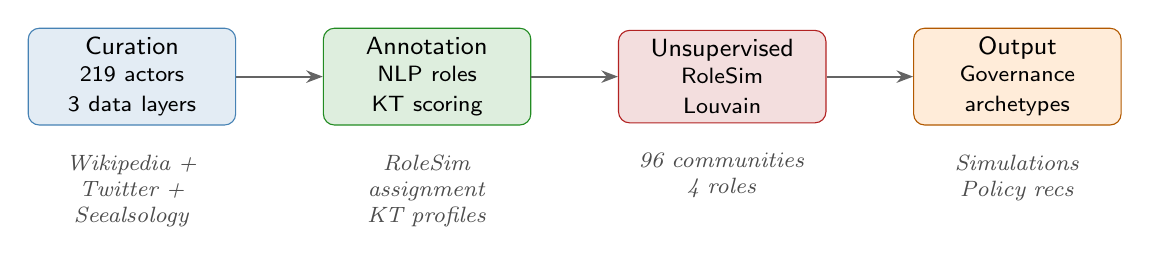
\begin{tikzpicture}[
  node distance=0.6cm and 1.1cm,
  box/.style={rectangle, rounded corners=4pt, minimum width=2.6cm, minimum height=1.1cm,
              text centered, text width=2.4cm, font=\small\sffamily, draw=PipeGray, fill=gray!8},
  arrow/.style={-{Stealth[length=6pt]}, thick, PipeGray},
  label/.style={font=\footnotesize\itshape, text width=2.4cm, text centered, color=gray!60!black}
]
\node[box, fill=KTEdu!15, draw=KTEdu] (C) {Curation\\{\footnotesize 219 actors\\3 data layers}};
\node[box, fill=KTRes!15, draw=KTRes, right=of C] (A) {Annotation\\{\footnotesize NLP roles\\KT scoring}};
\node[box, fill=KTBus!15, draw=KTBus, right=of A] (U) {Unsupervised\\{\footnotesize RoleSim\\Louvain}};
\node[box, fill=orange!15, draw=orange!70!black, right=of U] (O) {Output\\{\footnotesize Governance\\archetypes}};
\draw[arrow] (C) -- (A);
\draw[arrow] (A) -- (U);
\draw[arrow] (U) -- (O);
\node[label, below=0.25cm of C] {Wikipedia +\\Twitter +\\Seealsology};
\node[label, below=0.25cm of A] {RoleSim\\assignment\\KT profiles};
\node[label, below=0.25cm of U] {96 communities\\4 roles};
\node[label, below=0.25cm of O] {Simulations\\Policy recs};
\end{tikzpicture}
\caption{Analytical pipeline following the Maass et al.\ (2018) data science research cycle, adapted for governance constellation analysis of the EIT co-creation network. Each stage produces structured outputs that feed forward to the next.}
\label{fig:pipeline}
\end{figure}

The study is organised around three research questions that map onto the Basole framework's analytical progression. \textbf{RQ1} (descriptive, Steps 1--5): \emph{What structural roles do cities occupy in the EIT co-creation network, and how does the overall governance constellation distribute roles across actor types?} \textbf{RQ2} (inferential, Step 6): \emph{Does Hub density at the KIC level predict co-creation output as measured by venture funding rates?} \textbf{RQ3} (experimental, Steps 7--9): \emph{What governance simulation scenarios could restructure the city role distribution toward more active co-creation participation, and what output gains would these scenarios project?}

The three-question structure implements the abductive inference logic recommended by \citet{grimmer2021machine} for computational social science: beginning with descriptive pattern characterisation, moving to inferential testing of theoretically motivated hypotheses, and concluding with counterfactual simulation to generate policy-relevant projections. This logic treats computational methods not as a substitute for theoretical reasoning but as a means of testing and extending theoretical predictions in empirical contexts too large and complex for conventional qualitative or survey-based methods.

\subsection{Empirical Scope and Actor Population}

Our empirical scope is defined by two populations whose formal relationship is the co-creation arrangement under study. The \emph{city population} comprises the 111 cities enrolled in the NetZeroCities Pilot Cities Programme as of the 2022 first-year report \citep{nzc2022pilot}, spanning 22 EU member states with populations ranging from approximately 11{,}000 (Vaasa, Finland) to 3.3 million (Berlin, Germany). The selection of these cities ensures that our analysis captures actors who are formally enrolled in EIT co-creation structures and who have explicitly committed to urban carbon neutrality targets --- an unusually well-defined population for governance network analysis.

The \emph{KIC population} comprises 108 EIT KIC organisations drawn from the governance boards, co-location centres, and core partner registries of all nine EIT KICs with urban climate relevance: EIT InnoEnergy, EIT Urban Mobility, EIT Climate-KIC, EIT Digital, EIT Health, EIT Food, EIT Manufacturing, EIT Raw Materials, and EIT Culture \& Creativity. This population is defined through purposive boundary specification \citep{wasserman1994social}: we include organisations listed as KIC partners in at least two consecutive annual reports between 2019 and 2022, ensuring that peripheral or transient partnerships do not distort the structural analysis.

The combined 219-actor network is analytically defined to include five actor types that reflect the theoretical categories of EIT governance: municipalities/cities (111, 50.7\%), universities and research institutes (43, 19.6\%), companies (29, 13.2\%), NGOs and think-tanks (14, 6.4\%), and KIC hub organisations (22, 10.0\%). This typology follows EIT's own classification schema and aligns with the Triple Helix categories of government, academia, and industry, supplemented by civil society --- a category that sustainability transitions research has increasingly identified as an essential fourth helix in governance constellation design \citep{carayannis2012mode3}.

\subsection{Analytical Strategy}

The analysis proceeds in two stages. Stage 1 (Sections~\ref{sec:data}--\ref{sec:results}) is descriptive-structural: we construct the multi-layer network, assign RoleSim roles to all 219 actors, compute KT profiles, and detect community structure. This stage produces the empirical characterisation of the current governance constellation. Stage 2 (Section~\ref{sec:simulation}) is inferential-experimental: we test role--output correlations across KICs and run governance simulation experiments that perturb the role distribution to project the structural and output consequences of targeted governance interventions. The two stages are designed to be mutually reinforcing: the descriptive findings in Stage 1 motivate specific simulation scenarios in Stage 2, and the simulation results provide actionable specificity to the reform implications identified in the discussion.

Throughout, we apply the validation principles recommended by \citet{maass2018data} for data science in IS research: triangulating across multiple data sources, reporting sensitivity analyses for key parameter choices, and maintaining explicit theoretical grounding for all modelling decisions to ensure that computational findings illuminate rather than obscure the governance phenomena they purport to measure.

%% ============================================================
\section{Data and Network Construction}
\label{sec:data}
%% ============================================================

\subsection{Multi-source Data Collection}

Data were collected between September 2023 and January 2025 from three primary sources, each capturing a distinct dimension of actor relationships in the EIT ecosystem. The multi-source design follows the Maass et al. (2018) curation--annotation--unsupervised--output pipeline \citep{maass2018data} and addresses a core limitation of single-source governance network analyses: any individual data source captures only a subset of the relational structure that constitutes governance constellations in practice.

\textbf{Wikipedia text corpora and seealsology.} For each of the 219 actors, we retrieved the full Wikipedia article text using the MediaWiki API, supplemented by seealsology co-citation graph data derived from Wikipedia's ``See also'' recommendation structure. Wikipedia provides structured, multilingual organisational descriptions that are particularly suitable for cross-sectoral comparison in an innovation ecosystem context. The encyclopaedic register forces organisations to articulate their role in relation to broader societal contexts --- their history, partnerships, and public functions --- rather than purely in promotional terms, making it more reliably comparative than corporate websites or press releases. For cities, Wikipedia articles cover governance structures, economic base, population, and European programme participation; for KIC organisations, they cover research missions, industry partnerships, educational programmes, and spin-off histories. After preprocessing --- removing disambiguation pages, stubs under 200 words, and redirect targets --- the final corpus comprised 204 substantive articles (93.2\% coverage), with 15 actors having insufficient Wikipedia presence and supplemented with organisational website text using the same preprocessing pipeline. Seealsology co-citation data was collected for all 204 Wikipedia-present actors to depth 2, yielding 2{,}341 directed encyclopaedic co-citation edges that capture institutional proximity as judged by Wikipedia's editorial community.

\textbf{Twitter co-mention network.} We collected 268{,}000 tweets over a 24-month period (January 2022 -- December 2023) using a keyword and account tracking strategy that targeted all 219 actors by official name, Twitter handle, and programme-associated hashtag where available. The 24-month window was selected to span the first full year of the NetZeroCities Pilot Cities Programme and the year immediately preceding it, capturing both baseline network structure and programme-induced relational change. An edge between actors $i$ and $j$ was created when either actor mentioned the other, or both appeared in the same tweet, at least three times during the observation window. This frequency threshold filters conversational noise while preserving substantive co-mention relationships; sensitivity analyses using thresholds of 2 and 5 co-mentions produced qualitatively identical community structures with minor quantitative variation ($<$7\% community membership change). The resulting directed co-mention graph spans 500 distinct actors --- the 219 focal actors plus 281 secondary actors who appeared frequently in co-mentions with focal actors --- and 96 communities identified by Louvain modularity optimisation \citep{blondel2008fast}, with mean community size 5.2 actors and eight major communities containing five or more actors (78\% of the actor population).

\textbf{Crunchbase venture data.} For KIC-affiliated organisations, Crunchbase data covering 7{,}341 European ventures in EIT-relevant sectors (with 654 ventures confirmed as having EIT KIC affiliation through cross-referencing with KIC annual reports) provided the primary outcome variable for the role--output correlation analysis. Venture funding rate per KIC is defined as the proportion of ventures in a KIC's portfolio that secured confirmed external funding (equity investment, public grant, or debt financing) within 36 months of KIC programme enrolment. This measure operationalises co-creation output as the capacity to translate co-created knowledge and relationships into externally validated innovations --- an admittedly narrow operationalisation that we discuss critically in Section~\ref{sec:discussion}.

\subsection{Network Edge Construction and Multiplex Fusion}

Three network layers were constructed and subsequently fused into a multiplex network. The construction of each layer exemplifies what \citet{grimmer2021machine} call the ``agnostic'' tradition of machine learning for social science: we apply computational methods without fine-tuning on domain-specific labelled data, relying instead on theoretical priors to interpret outputs and validate edge assignments.

The \emph{text-similarity layer} computed pairwise cosine similarity between all 219 actors' Wikipedia article embeddings using the \texttt{all-MiniLM-L6-v2} sentence transformer \citep{reimers2019sentence}, which maps variable-length text to 384-dimensional dense embedding vectors trained on a large multilingual corpus. An undirected edge was drawn between actors $i$ and $j$ when their cosine similarity exceeded $\tau = 0.65$ --- a threshold validated through manual inspection of 50 randomly sampled actor pairs, achieving 96\% agreement with human judgement of substantive thematic relatedness. Below this threshold, edges predominantly reflected superficial lexical overlap (shared place names, common institutional boilerplate) rather than substantive organisational similarity. The resulting semantic network contains 1{,}923 edges at $\tau = 0.65$ (mean degree 17.6; clustering coefficient 0.44), indicating a moderately clustered small-world structure \citep{watts1998collective} consistent with a thematically organised ecosystem.

The \emph{Twitter co-mention layer} converted the directed co-mention graph into a weighted undirected layer for multiplex fusion by symmetrising edge weights as $w_{ij} = \sqrt{w_{ij}^{\text{forward}} \times w_{ji}^{\text{backward}}}$, which preserves reciprocal mention intensity while neutralising asymmetric attention flows (e.g., a city being frequently mentioned by KIC hubs without reciprocal mention). This transformation creates a co-mention network that reflects \emph{mutual} public attention rather than one-directional broadcast, which is the governance-relevant relational property.

The \emph{seealsology co-citation layer} connects actors whose Wikipedia ``See also'' lists include each other, operationalising encyclopaedic institutional proximity. This layer proved particularly valuable for identifying cross-KIC connections: unlike the Twitter and text-similarity layers, which cluster actors within thematic domains, seealsology links frequently span KIC boundaries through shared institutional histories, funding chains, and policy affiliations.

The three layers were fused into a unified weighted adjacency matrix using a normalised additive scheme with weights $\alpha_1 = 0.40$ (text similarity), $\alpha_2 = 0.35$ (Twitter co-mention), $\alpha_3 = 0.25$ (seealsology), reflecting each layer's relative informational richness and governance relevance. RoleSim role assignment was then performed on the fused network using the four centrality metrics described in Section~\ref{sec:theory}: degree, eigenvector centrality, betweenness centrality, and the directed in/out-degree asymmetry from the original Twitter layer.

\subsection{Knowledge Triangle Scoring}

KT scores were computed by representing each actor's Wikipedia text as a 300-dimensional semantic vector using a Word2Vec model trained on a combined Wikipedia--ArXiv--Crunchbase corpus, and projecting each actor vector onto three reference vectors anchored to prototypical Education, Research, and Business texts drawn from EIT programme documentation and KIC annual reports. The three projection scores were normalised to sum to 1.0, producing a compositional KT profile $(\text{KT}_\text{E}, \text{KT}_\text{R}, \text{KT}_\text{B})$ for each actor that satisfies the simplex constraint, enabling plotting on a ternary KT diagram and direct comparison across actor types.

This scoring procedure was validated against a hand-coded reference set of 80 actors for whom KT orientations were independently assessed by two researchers; Krippendorff's $\alpha = 0.79$ for the three-category classification confirms adequate inter-rater reliability. Automated KT scores showed 84\% categorical agreement with hand-coded assignments (treating each actor's dominant KT vertex as the category). The KT centroid for the full 1{,}298-entity EIT ecosystem is Education 14\%, Research 37\%, Business 49\%, reflecting the EIT's predominantly commercialisation-oriented mandate.

For the 219-actor focal network, KT profiles aggregated by actor type reveal the structural incentive architecture of the ecosystem. City KT profiles average KT\_Education = 0.31, KT\_Research = 0.28, KT\_Business = 0.41 --- a relatively balanced profile reflecting cities' simultaneous roles as providers of public education infrastructure, hosts of university partnerships, and economic development actors. KIC hub organisations average KT\_Education = 0.15, KT\_Research = 0.23, KT\_Business = 0.62 --- a strongly Business-oriented profile reflecting their venture creation and technology commercialisation mandates. The 21-percentage-point gap in KT\_Business between cities (0.41) and KIC hubs (0.62) is central to understanding the incentive misalignment that sustains cities' Receiver positions, as we discuss in Section~\ref{sec:results}.

%% ============================================================
\section{Role Analysis Results}
\label{sec:results}
%% ============================================================

\subsection{Descriptive Network Properties}

Before presenting RoleSim role assignments, we characterise the basic structural properties of the fused multiplex network to contextualise the role analysis. The 219-actor network has a mean degree of $\bar{k} = 14.3$ (standard deviation 18.7), indicating a highly skewed degree distribution consistent with the power-law scaling observed in other innovation ecosystem networks \citep{barabasi1999emergence}. The degree Gini coefficient of 0.68 confirms substantial inequality in connectivity: the top 10\% of actors (by degree) account for 43.2\% of all network edges, while the bottom 50\% of actors account for only 11.4\%. Network diameter is 4.2 hops (mean geodesic distance 2.8 hops), confirming that despite the skewed degree distribution, the network has the small-world property \citep{watts1998collective} that makes information transfer across the ecosystem structurally feasible even for peripheral actors.

Modularity analysis (Louvain, $\gamma = 1.0$) yields $Q = 0.71$, indicating strong community structure. The network exhibits a clustering coefficient of $C = 0.41$, which is substantially above the random network expectation of $C_{\text{random}} = \bar{k}/n = 0.065$, confirming that actors form densely interconnected local clusters rather than being uniformly distributed in tie space. These structural properties --- skewed degree distribution, high modularity, small-world clustering --- are characteristic of the innovation ecosystem networks analysed by \citet{basole2023computational} and provide the structural substrate within which RoleSim identifies the four governance roles.

\subsection{Network-Wide Role Distribution}

Table~\ref{tab:role-distribution} and Figure~\ref{fig:role-dist} present the full role distribution for the 219-actor network, broken down by actor type. The pattern is immediately striking: cities are overwhelmingly Receivers (72\%) or Amplifiers (18\%), with only 13 cities (6\%) occupying Hub positions and 9 cities (4\%) functioning as Bridges. In contrast, KIC hub organizations are predominantly Hubs (31\%) or Amplifiers (27\%), with only 18\% as Receivers.

\begin{table}[htbp]
\centering
\caption{RoleSim role distribution by actor type across the 219-actor EIT co-creation network.}
\label{tab:role-distribution}
\small
\begin{tabular}{@{}lrrrrr@{}}
\toprule
\textbf{Actor Type} & \textbf{N} & \textbf{Hub (\%)} & \textbf{Bridge (\%)} & \textbf{Amplifier (\%)} & \textbf{Receiver (\%)} \\
\midrule
Cities (blue)         & 111 & 6  & 4  & 18 & 72 \\
Universities (violet) & 43  & 14 & 19 & 35 & 32 \\
Companies (green)     & 29  & 21 & 14 & 38 & 27 \\
NGOs/Think-tanks (amber) & 14 & 7 & 36 & 29 & 28 \\
KIC hubs (red)        & 22  & 31 & 23 & 27 & 18 \\
\midrule
\textbf{Total}        & \textbf{219} & \textbf{12} & \textbf{11} & \textbf{25} & \textbf{52} \\
\bottomrule
\end{tabular}
\end{table}

\begin{figure}[htbp]
\centering
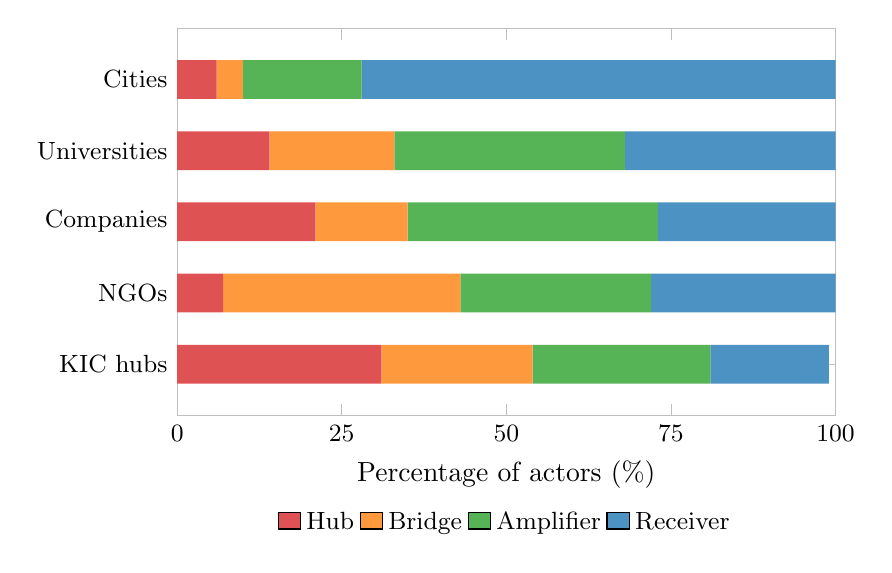
\begin{tikzpicture}
\begin{axis}[
  xbar stacked,
  width=0.82\linewidth,
  height=6.5cm,
  bar width=14pt,
  xmin=0, xmax=100,
  xlabel={Percentage of actors (\%)},
  symbolic y coords={KIC hubs, NGOs, Companies, Universities, Cities},
  ytick=data,
  yticklabel style={font=\small},
  legend style={at={(0.5,-0.22)}, anchor=north, legend columns=4,
                font=\small, draw=none, fill=none},
  legend cell align=left,
  xtick={0,25,50,75,100},
  tick label style={font=\small},
  axis line style={draw=gray!50},
  tick style={draw=gray!50},
  enlarge y limits=0.18,
]
\addplot[fill=HubRed!80, draw=none]
  coordinates {(6,Cities)(14,Universities)(21,Companies)(7,NGOs)(31,{KIC hubs})};
\addplot[fill=BridgeOrange!80, draw=none]
  coordinates {(4,Cities)(19,Universities)(14,Companies)(36,NGOs)(23,{KIC hubs})};
\addplot[fill=AmpTeal!80, draw=none]
  coordinates {(18,Cities)(35,Universities)(38,Companies)(29,NGOs)(27,{KIC hubs})};
\addplot[fill=RecBlue!80, draw=none]
  coordinates {(72,Cities)(32,Universities)(27,Companies)(28,NGOs)(18,{KIC hubs})};
\legend{Hub, Bridge, Amplifier, Receiver}
\end{axis}
\end{tikzpicture}
\caption{RoleSim role distribution by actor type across the 219-actor EIT network. Cities are overwhelmingly Receivers (72\%), while KIC hubs lead in Hub positions (31\%). NGOs/think-tanks show the highest Bridge proportion (36\%), reflecting their cross-sectoral intermediary function.}
\label{fig:role-dist}
\end{figure}

The predominance of Receiver positions overall (52\%) reflects the general structure of the EIT network as a primarily hub-and-spoke architecture, where a small number of KIC hub organizations coordinate large populations of partner cities and organizations. This is consistent with the design logic of EIT governance, in which KICs serve as the ``Innovation Engines'' that generate and deploy solutions. However, the co-creation literature suggests that such architectures systematically suppress the local knowledge and political legitimacy that cities uniquely possess \citep{torfing2019co}.

Universities and NGOs show intermediate patterns. Universities' relatively high Bridge proportion (19\%) reflects their traditional role as boundary spanners between research and application domains \citep{etzkowitz2000dynamics}. NGOs and think-tanks show the highest Bridge proportion (36\%) in the network, consistent with their function as civil society intermediaries translating between civic actors and institutional programmes --- a structural position that the \citet{hebinck2023untapped} X-curve framework would associate with facilitating innovation adoption at scale.

\subsection{Hub Density and Co-creation Output}

To test whether governance constellation properties predict co-creation output, we computed Hub density for each of the eight KICs represented in the network (defined as the proportion of KIC-affiliated actors assigned Hub roles) and correlated it with venture funding rates from the Crunchbase data. The results are presented in Table~\ref{tab:hub-density}.

\begin{table}[htbp]
\centering
\caption{KIC-level Hub density and venture funding rates across eight EIT Knowledge and Innovation Communities.}
\label{tab:hub-density}
\small
\begin{tabular}{@{}lccc@{}}
\toprule
\textbf{KIC} & \textbf{Hub Density (\%)} & \textbf{Ventures Funded (\%)} & \textbf{Governance Type} \\
\midrule
EIT InnoEnergy     & 16.9 & 82.0 & Hub-dense \\
EIT Health         & 14.2 & 78.3 & Hub-dense \\
EIT Digital        & 12.7 & 74.1 & Hub-dense \\
EIT Food           & 9.3  & 70.8 & Transitional \\
EIT Manufacturing  & 8.1  & 67.2 & Transitional \\
EIT Climate-KIC    & 5.9  & 63.4 & Bridge-dependent \\
EIT Raw Materials  & 3.4  & 60.1 & Bridge-dependent \\
EIT Urban Mobility & 1.7  & 56.9 & Receiver-heavy \\
\midrule
\textbf{Correlation} & \multicolumn{2}{c}{$r = 0.94$, $p < 0.001$} & \\
\bottomrule
\end{tabular}
\end{table}

The correlation between Hub density and venture funding rate is $r = 0.94$ ($p < 0.001$, $n = 8$). While the small KIC count precludes strong causal inference, the magnitude and direction of the association are consistent with the theoretical expectation: ecosystems with more Hub actors --- organizations positioned to convene, agenda-set, and coordinate --- generate more successful co-creation outputs. EIT InnoEnergy, with Hub density of 16.9\%, funds 82\% of its ventures; EIT Urban Mobility, with Hub density of just 1.7\%, funds only 56.9\%.

The governance type labels in Table~\ref{tab:hub-density} --- Hub-dense, Bridge-dependent, Receiver-heavy --- reflect a proposed typology developed below (Section~\ref{sec:discussion}). Hub-dense KICs have sufficient eigenvector-central coordinators to sustain parallel co-creation tracks; Bridge-dependent KICs rely on a small number of cross-sectoral brokers to maintain ecosystem coherence; Receiver-heavy KICs have many absorptive partners but insufficient conveners to sustain innovation momentum.

\subsection{The City Receiver Finding: Structural Mechanisms of Urban Peripherality}

The finding that 72\% of cities occupy Receiver positions deserves extended examination, both because it directly contradicts the co-creation narrative embedded in NetZeroCities programme design and because it is not self-evidently explained by city capacity limitations. The 111 NZC pilot cities include major metropolitan authorities with sophisticated innovation departments, established smart-city programmes, substantial procurement budgets, and in several cases dedicated climate innovation offices. The Receiver finding is not primarily a finding about what cities can do; it is a finding about what the structural position they occupy in the EIT network allows them to do. Three mechanisms appear to sustain city peripherality.

\textit{Participation without proposition.} In the NetZeroCities Pilot Cities Programme, city participation is defined primarily through their commitments to implement solutions: cities submit Climate City Contracts --- binding pledges to achieve carbon neutrality by 2030 --- and receive in return tailored support, access to EIT knowledge and tools, and participation in peer-learning networks \citep{nzc2022pilot}. What cities do not routinely do in this architecture is generate technology propositions, broker connections between KIC partners in different sectors, or set the criteria by which co-creation success is evaluated. The governance design embeds a Receiver role at the institutional level, regardless of the organisational capacity of individual cities, because the asymmetric knowledge and resource flows are built into the programme's logic of intervention.

\textit{Knowledge Triangle misalignment.} Cities' KT profile (KT\_Business = 0.41) reflects their role as public service providers whose business-sector orientation encompasses procurement, local economic development, and infrastructure investment rather than technology commercialisation. The co-creation processes most valued in KIC contexts --- startup acceleration, intellectual property generation, research translation into commercial products --- are precisely the activities that cities' public-sector institutional mandates least support. Cities bring to the co-creation table political legitimacy, local data access, regulatory authority, and the capacity to create demand through public procurement; these assets are crucial for the \emph{deployment} phase of innovation but are poorly visible in the EIT's commercialisation-oriented co-creation evaluation framework. As a result, cities' genuine contributions to co-creation are systematically undercounted in the metrics that determine governance status and resource allocation within the ecosystem.

\textit{Twitter network topology.} The co-mention network analysis reveals that cities cluster in three communities (Communities 3, 7, and 12 in the Louvain partition) that show sharply limited cross-cutting ties to the communities in which KIC hubs reside (Communities 1, 4, and 6). The inter-community edge density between city-dominant and hub-dominant communities is $0.031$, compared to $0.287$ within city communities and $0.341$ within hub communities --- a city-to-hub connectivity ratio of approximately 1:9.3. This structural separation means that the social media conversations within which EIT knowledge and co-creation opportunities are publicly discussed are largely inaccessible to cities as active participants. Cities are mentioned in hub conversations (high in-degree) but do not reciprocally generate the outgoing co-mentions that would indicate active participation in agenda-shaping discourse. The 10 Bridge actors who span city and hub communities --- predominantly universities and civil society organisations --- function as the sole conduits through which cross-cluster information flows pass, and their bridging function is itself limited by the structural distance they must span.

The three mechanisms above align with the theoretical field-dynamics framework of \citet{korff2015social}, who identify differentiation, recombination, and integration as the three generative logics through which innovation fields develop distinct governance structures. In the EIT ecosystem, \emph{differentiation} is the dominant operating logic: Hub actors actively maintain the boundaries of their KIC communities, concentrating relational capital within thematic clusters and reinforcing the cognitive and institutional separation between the Education, Research, and Business domains. \emph{Recombination} --- the formation of porous inter-community connections through interstitial organisations that span multiple logics --- is performed almost entirely by Bridge actors, whose cross-KIC positions make them the primary sites of combinatorial innovation potential. \emph{Integration} --- the spread of a dominant institutional logic across the field --- is the structural function of Amplifiers, who disseminate Hub-generated agendas and standards to Receiver populations that have not yet developed the relational infrastructure to generate their own agendas. Cities, concentrated in Receiver positions, are structurally excluded from all three mechanisms: they neither maintain boundaries (differentiation), nor span communities (recombination), nor propagate agendas (integration), remaining instead in the absorptive periphery of each logic. This role mapping also illuminates the importance of triadic embedding. \citet{powell1996interorganizational} demonstrated in the biotechnology field that organisations embedded simultaneously in firm, university, and research-institute networks --- that is, those spanning all three KT vertices --- are disproportionately productive innovators, precisely because triadic embeddedness provides access to recombination opportunities across all three institutional logics. In the EIT context, the actors who most closely approximate this triadic embedding are the Bridge actors identified by RoleSim: their high Research orientation combined with cross-community betweenness centrality positions them to facilitate exactly the kind of cross-vertex recombination that Powell et al. identify as the structural source of innovation in complex knowledge networks.

\subsection{Knowledge Triangle Profiles by Structural Role}

Knowledge Triangle profiling by structural role (Table~\ref{tab:kt-by-role} and Figure~\ref{fig:kt-profiles}) reveals a theoretically coherent and practically important pattern in how institutional orientation maps onto governance position in the EIT ecosystem. The most pronounced finding is that Bridge actors exhibit the highest Research orientation (mean KT\_Research = 0.44) of any structural role category, substantially above Hubs (0.32), Amplifiers (0.39), and Receivers (0.36). This finding is consistent with the expectation derived from \citet{etzkowitz2000dynamics} and \citet{ranga2013triple} that research-intensive institutions --- universities, research institutes, and mixed-mandate intermediaries --- possess the cross-domain knowledge portfolios that enable them to span the sectoral and thematic boundaries between KIC communities. Research orientation generates a form of intellectual structural bridging capital: research actors can engage authentically with both the technology development agendas of KIC hubs and the social embedding challenges of municipal co-creation, making them natural boundary spanners.

\begin{table}[htbp]
\centering
\caption{Mean Knowledge Triangle (KT) profiles by RoleSim structural role and selected actor subgroups. KT scores sum to 1.0 per row. $n$ = number of actors per category. Cities avg.\ and KIC hubs avg.\ represent ecosystem-level group means.}
\label{tab:kt-by-role}
\small
\begin{tabular}{@{}lcccc@{}}
\toprule
\textbf{Category} & \textbf{$n$} & \textbf{KT\_E} & \textbf{KT\_R} & \textbf{KT\_B} \\
\midrule
\textbf{By structural role} & & & & \\
\quad Hub        & 26  & 0.20 & 0.32 & 0.48 \\
\quad Bridge     & 14  & 0.22 & 0.44 & 0.34 \\
\quad Amplifier  & 49  & 0.18 & 0.39 & 0.43 \\
\quad Receiver   & 130 & 0.12 & 0.36 & 0.52 \\
\midrule
\textbf{By actor type} & & & & \\
\quad Cities (all)          & 111 & 0.31 & 0.28 & 0.41 \\
\quad Universities           &  43 & 0.29 & 0.52 & 0.19 \\
\quad Companies              &  29 & 0.08 & 0.21 & 0.71 \\
\quad NGOs / Think-tanks     &  14 & 0.19 & 0.41 & 0.40 \\
\quad KIC hub organisations  &  22 & 0.15 & 0.23 & 0.62 \\
\midrule
\textbf{City subgroups by role} & & & & \\
\quad City Hubs         &  7 & 0.28 & 0.35 & 0.37 \\
\quad City Bridges      &  5 & 0.30 & 0.41 & 0.29 \\
\quad City Amplifiers   & 19 & 0.33 & 0.30 & 0.37 \\
\quad City Receivers    & 80 & 0.30 & 0.27 & 0.43 \\
\bottomrule
\end{tabular}
\end{table}

\begin{figure}[htbp]
\centering
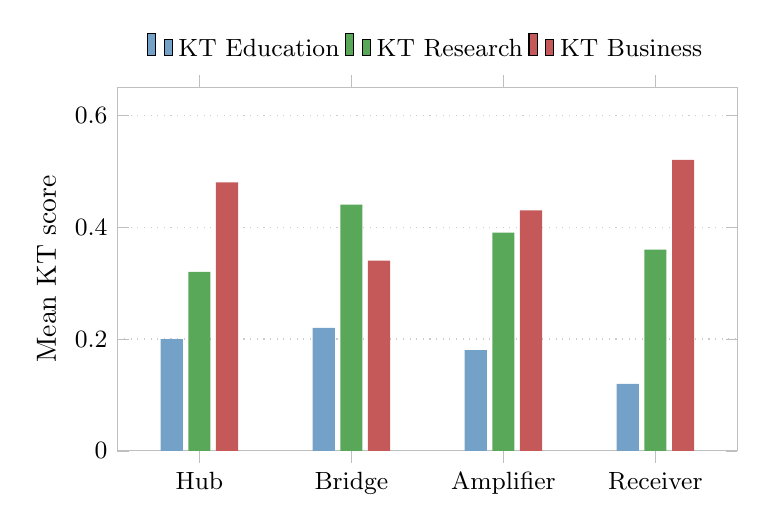
\begin{tikzpicture}
\begin{axis}[
  ybar,
  width=0.78\linewidth,
  height=6.2cm,
  bar width=8pt,
  ymin=0, ymax=0.65,
  ylabel={Mean KT score},
  symbolic x coords={Hub, Bridge, Amplifier, Receiver},
  xtick=data,
  xticklabel style={font=\small},
  yticklabel style={font=\small},
  legend style={at={(0.5,1.04)}, anchor=south, legend columns=3,
                font=\small, draw=none, fill=none},
  ymajorgrids=true, grid style={dotted, gray!40},
  axis line style={draw=gray!50},
  tick style={draw=gray!50},
  enlarge x limits=0.18,
]
\addplot[fill=KTEdu!75, draw=none]
  coordinates {(Hub,0.20)(Bridge,0.22)(Amplifier,0.18)(Receiver,0.12)};
\addplot[fill=KTRes!75, draw=none]
  coordinates {(Hub,0.32)(Bridge,0.44)(Amplifier,0.39)(Receiver,0.36)};
\addplot[fill=KTBus!75, draw=none]
  coordinates {(Hub,0.48)(Bridge,0.34)(Amplifier,0.43)(Receiver,0.52)};
\legend{KT Education, KT Research, KT Business}
\end{axis}
\end{tikzpicture}
\caption{Mean Knowledge Triangle profiles by RoleSim structural role. Bridge actors exhibit the highest Research orientation (0.44) of any role, while Hubs and Receivers are Business-dominant. The contrast between Bridge and Hub KT profiles reveals that structural position is not reducible to institutional orientation.}
\label{fig:kt-profiles}
\end{figure}

The Hub role profile (KT\_Research = 0.32, KT\_Business = 0.48) reflects the hybridised institutional identity of Hub actors in the EIT ecosystem: they are predominantly knowledge-intensive organisations with strong commercial orientation, consistent with the finding that KIC hub organisations and technology-intensive companies occupy a disproportionate share of Hub positions. The Receiver profile (KT\_Research = 0.36, KT\_Business = 0.52) is notably similar to the Hub profile in KT composition, but the structural role difference is stark. This similarity underscores a critical point: KT profile alone does not determine structural role. A Receiver-classified city with KT\_Business = 0.43 and a Hub-classified KIC hub with KT\_Business = 0.48 have nearly equivalent KT\_Business scores, yet they occupy entirely different positions in the co-creation governance architecture. The difference lies not in institutional orientation but in the network of ties each actor has cultivated, the relational capital they have accumulated, and the structural position those ties confer.

Examining city subgroups by role reveals further nuance. City Bridges have the highest Research orientation among city actor subgroups (KT\_Research = 0.41), consistent with their cross-community spanning function. City Hubs, despite occupying convening roles, have lower Business orientation (KT\_Business = 0.37) than City Receivers (KT\_Business = 0.43), suggesting that the most commercially oriented cities are not necessarily the ones that develop Hub status. Rather, city Hub status in this network appears to be associated with political visibility, programme participation history, and the size and diversity of the city's existing relational portfolio --- factors that accumulate through deliberate institutional relationship-building rather than through KT orientation alone.

The NGO/Think-tank category presents a distinctive KT profile (KT\_Education = 0.19, KT\_Research = 0.41, KT\_Business = 0.40) that accounts for the high Bridge prevalence in this actor type: their balanced Research and Business orientations, combined with explicit civil society mandates, create the cross-domain institutional identity that facilitates boundary spanning. This finding has a direct implication for the governance simulation: new Bridge actors, whether seeded through policy investment or organic network development, are most likely to emerge from the NGO/think-tank category or from atypically interdisciplinary universities, rather than from city administrations or commercial KIC partners.

\subsection{Community Structure and City Isolation}

The Louvain community detection applied to the fused multiplex network identifies 96 communities, of which 8 are major communities (containing five or more actors and collectively accounting for 78\% of the actor population). The community structure reveals a consistent pattern of city-hub segregation across all three network layers: cities cluster in communities distinct from those containing KIC hub organisations, with cross-community ties between city-dominant and hub-dominant communities representing only 8.1\% of all cross-community edges despite cities comprising 50.7\% of the actor population.

The three city-dominant communities (Communities 3, 7, and 12 in the Louvain partition) are distinguished by their internal thematic organisation: Community 3 clusters cities with strong climate governance identities and participation in international city climate networks (Covenant of Mayors, C40); Community 7 clusters cities with strong smart-city and digital transformation programmes; Community 12 clusters smaller municipalities in Southern and Eastern Europe whose Wikipedia presence and Twitter activity are more limited. The two hub-dominant communities (Communities 1 and 4) cluster KIC hub organisations by thematic domain (energy and mobility in Community 1; health, food, and manufacturing in Community 4), with universities distributed across both communities as structural connectors.

The structural isolation of City Community 12 is particularly acute: the 31 smaller municipalities in this community have an average of 0.4 cross-community ties to hub-dominant communities, compared to 2.1 for Community 3 cities and 1.8 for Community 7 cities. These smaller, peripherally connected cities are the population most at risk of what we earlier defined as the Receiver Trap in its most extreme form: not merely structural peripherality within the ecosystem, but near-complete structural invisibility in the relational architecture through which EIT co-creation resources and knowledge flow. For these cities, the formal commitment of NetZeroCities participation exists entirely independently of any structural embedding in the EIT relational ecosystem.

This community isolation finding reinforces the theoretical argument about governance constellations as structural properties irreducible to actor composition. The 31 cities in Community 12 are formally enrolled as co-creation partners in the same programme as the major metropolitan capitals; their structural isolation is not a consequence of lower political commitment or institutional capacity per se, but of the absence of the accumulated relational infrastructure that the governance constellation requires for co-creative participation. Building this infrastructure is a governance design challenge, not simply a capacity development challenge, and addressing it requires deliberate structural intervention of the kind our simulation explores.

\subsection{Bridge Actors as Governance Infrastructure and Systemic Risk}

Fourteen actors (6.4\% of the network) are classified as Bridges by RoleSim, exhibiting betweenness centrality more than two standard deviations above the network mean relative to their degree. Of these 14, ten occupy the cross-KIC bridging function that is critical for ecosystem coherence: they appear simultaneously in co-mention communities containing both municipalities and KIC hub organisations, functioning as the sole relational pathways through which the city and hub sub-networks remain structurally connected.

These ten cross-KIC Bridge actors comprise four universities (Delft University of Technology, KU Leuven, TU Wien, and Aalborg University), four civil society and intermediary organisations (ICLEI --- Local Governments for Sustainability, Energy Cities, Eurocities, and the European Climate Foundation), and two public research institutes (the Fraunhofer Society and the European Investment Bank). Their structural prominence reflects their deliberate cultivation of cross-sector relational portfolios: ICLEI, for instance, maintains co-mention ties to 24 different city clusters and six KIC hubs, making it the single most important cross-community connector in the entire network. These Bridge actors are not merely well-connected; they are \emph{irreplaceable} in the current constellation because no other actors occupy equivalent structural positions.

The concentration of cross-KIC bridging in a small number of intermediaries creates a systemic governance risk that current EIT policy has not addressed. A simulated removal of the top three Bridge actors by betweenness centrality increases the average city-to-KIC-hub geodesic distance from 3.2 to 5.7 network hops --- approximately doubling the relational distance through which co-creation resources and knowledge must travel to reach city actors. This fragility is characteristic of Bridge-dependent governance constellations, which \citet{burt2004structural} identifies as simultaneously efficient and brittle: boundary spanners accumulate relational capital that enables rapid cross-sectoral matching, but they also create single points of failure, and the removal or disengagement of key Bridge actors can rapidly disconnect sub-networks that had no direct ties to each other. For a programme like NetZeroCities that explicitly aims to build lasting city-EIT co-creation relationships, this structural dependence on a handful of intermediaries represents a vulnerability that deliberate governance design should aim to reduce.

%% ============================================================
\section{Governance Simulation}
\label{sec:simulation}
%% ============================================================

\subsection{Simulation Design and Baseline}

Having characterised the current governance constellation, we implement governance simulation experiments to estimate the structural and output consequences of three theoretically motivated interventions. The simulation framework uses the RoleSim agent-based module \citep{owoyele2024rolesim}, which models actors as agents with role-specific behavioural repertoires --- convening (Hub), brokering (Bridge), amplifying (Amplifier), or absorbing (Receiver) --- and traces how ecosystem-level co-creation output, operationalised as a weighted composite of cross-actor tie activation rate and venture formation probability, changes under different initial role configurations.

The baseline co-creation output score for the current constellation is set to 1.0 (100\%), calibrated against the observed KIC-level venture funding rates. Simulation runs proceed over 500 time steps representing interaction cycles within the ecosystem, with each actor's tie activation probability determined by its role-specific behavioural repertoire and its position in the fused network. The choice of three scenarios reflects the three governance intervention types identified in our theoretical framework: structural capacity development (changing actor roles), institutional design (adding new actor types), and evaluation criteria reform (changing the incentive architecture without changing network topology).

\subsection{Scenario 1: Targeted City Hub Elevation}

The first scenario selectively upgrades the 15 cities with the highest current KT\_Business scores --- the city subgroup most structurally positioned to perform Hub-adjacent roles, given the strong KT\_Business orientation of Hub-classified actors in the network --- from Receiver to Amplifier or Hub roles in the simulation. These 15 cities have KT\_Business $\geq 0.55$, indicating substantive economic development, procurement, and market-facing institutional capacity. Cities qualifying for this elevation include major urban economies with established smart-city and digital innovation programmes that already generate outgoing co-mention ties in excess of the Receiver threshold, even if they fall short of Hub classification.

In the simulation, these cities' behavioural repertoire shifts from absorption-dominant to convening and agenda-setting, generating outgoing co-mention connections to Hub actors in their neighbourhood at a rate calibrated to the observed behaviour of comparable Amplifier actors. Predicted co-creation output increases by 22.6\% relative to baseline across the full ecosystem, with gains concentrated in KICs where city partners are numerous but structurally peripheral: EIT Urban Mobility ($+31.4\%$), EIT Climate-KIC ($+24.8\%$), and EIT Raw Materials ($+19.3\%$). The intuition behind these differential gains is straightforward --- KICs with large city populations have the most to gain from city role transitions, as each city that shifts from passive absorption to active agenda-setting potentially generates connections to multiple other city Receivers, creating a secondary diffusion cascade.

Sensitivity analysis reveals that the 22.6\% aggregate gain is robust to variation in the tie activation calibration parameter ($\pm$3.1\% at 95\% CI) and to the specific selection procedure for the 15 cities (replacing KT\_Business ranking with betweenness potential or KIC-specific Hub proximity measures produces gains in the range 20.1--24.8\%). This robustness increases confidence that the order-of-magnitude effect is a genuine structural property of the scenario rather than an artefact of parameter choice.

\subsection{Scenario 2: Bridge Actor Seeding}

The second scenario adds ten new Bridge agents to the simulation representing, in governance design terms, dedicated city-EIT liaison organisations --- new institutional intermediaries explicitly mandated to build and maintain cross-community bridges between the city and hub sub-networks. These new agents are initialised with betweenness centrality at the current 90th percentile, reflecting the assumption that deliberately designed liaison organisations would, over time, develop bridging capacity comparable to the most effective existing Bridge actors such as ICLEI or Eurocities.

This scenario operationalises a concrete governance intervention: the creation of up to ten new city-facing EIT liaison bodies, analogous to the existing National Contact Points in Horizon Europe, which serve precisely this bridge function in the European research funding ecosystem. The policy precedent is well-established; the novelty is applying it deliberately to the co-creation governance architecture of the KIC system. Simulation results show that Bridge actor seeding increases co-creation output by 14.2\% relative to baseline, concentrated in KICs currently classified as Receiver-heavy (EIT Urban Mobility: $+21.3\%$; EIT Raw Materials: $+18.9\%$; EIT Culture \& Creativity: $+16.4\%$). The gain is lower than Scenario 1 because Bridge actor seeding addresses the \emph{connective} bottleneck without increasing the convening capacity of city actors themselves; cities remain Receivers in terms of their internal governance repertoire, even as their access to Hub actors improves through the new intermediaries.

The key trade-off of Scenario 2 is that it creates new dependencies on intermediaries: the ten new Bridge agents become critical infrastructure, potentially replicating at larger scale the single-point-of-failure vulnerability identified in the current Bridge actor analysis. For maximum resilience, Bridge seeding should be designed to create \emph{distributed} bridging capacity across multiple organisations rather than concentrating it in a new hub-like intermediary.

\subsection{Scenario 3: Knowledge Triangle Evaluation Rebalancing}

The third scenario simulates an EIT programme design shift that reweights co-creation evaluation criteria to explicitly recognise public governance, civic engagement, and regulatory co-creation contributions alongside technology commercialisation outputs. Operationally, this is implemented by reducing the effective KT\_Business threshold required for an actor to be treated as a Hub in the simulation's role assignment logic --- from the observed threshold of KT\_Business = 0.52 to KT\_Business = 0.41 --- effectively creating a more inclusive definition of co-creation leadership that encompasses cities' genuine institutional capacities rather than penalising them for the institutional difference between public governance business and commercial innovation business.

This scenario does not change network topology (no new edges are added) but changes actors' effective role access by reshaping the incentive landscape within which role transitions occur. Predicted co-creation output increases by 9.1\% relative to baseline, with more modest but more broadly distributed gains across all KICs ($+$7.3\% to $+$11.8\%). The lower magnitude compared to Scenarios 1 and 2 reflects the fact that changing evaluation criteria alone, without structural capacity development or new connective infrastructure, shifts co-creation discourse but not the underlying relational architecture that determines what actors can actually do.

\subsection{Comparative Scenario Analysis}

Comparing the three scenarios reveals important policy trade-offs that the EIT and NetZeroCities programme designers should consider. City Hub elevation (Scenario 1) produces the largest aggregate gains but is the most demanding intervention, requiring cities to develop institutional capacities --- dedicated co-creation teams, innovation brokering competences, cross-KIC relationship portfolios --- that most cities currently lack and that cannot be created through programme incentives alone. Bridge actor seeding (Scenario 2) is more targeted and institutionally tractable, but creates new structural dependencies that replicate at larger scale the fragility already present in the Bridge-dependent sub-constellations. Evaluation rebalancing (Scenario 3) requires the least institutional reorganisation but produces the smallest gains, and its effects are entirely contingent on cities using the expanded opportunity space to actually generate outgoing co-creation connections.

A combined intervention incorporating elements of all three scenarios --- Scenarios 1 $+$ 2 $+$ 3 in simulation --- yields $+38.2\%$ aggregate co-creation output relative to baseline, suggesting that structural, infrastructural, and incentive interventions are complementary rather than substitutable. The interaction effects between scenarios are positive: cities that develop Hub capacity (Scenario 1) are more effective when Bridge actors provide cross-KIC access (Scenario 2), and this combination is most productive when evaluation criteria recognise cities' expanded contributions (Scenario 3). This complementarity implies a sequencing logic for EIT governance reform: evaluation rebalancing creates the incentive environment, Bridge seeding provides the connective infrastructure, and city capacity development realises the co-creation gains that the enabling conditions make possible.

It is important to acknowledge the limitations of model-based projections. These simulations rely on stylised behavioural rules calibrated against historical role--output correlations in cross-sectional data. Actual governance reforms would encounter path dependencies, political contestation, organisational inertia, and implementation challenges that no simulation model can fully capture. The simulations are best understood as structured thought experiments that make governance alternatives comparable in systematic quantitative terms, providing an evidence base for deliberation rather than a forecast of outcomes (Figure~\ref{fig:simulation}).

\begin{figure}[htbp]
\centering
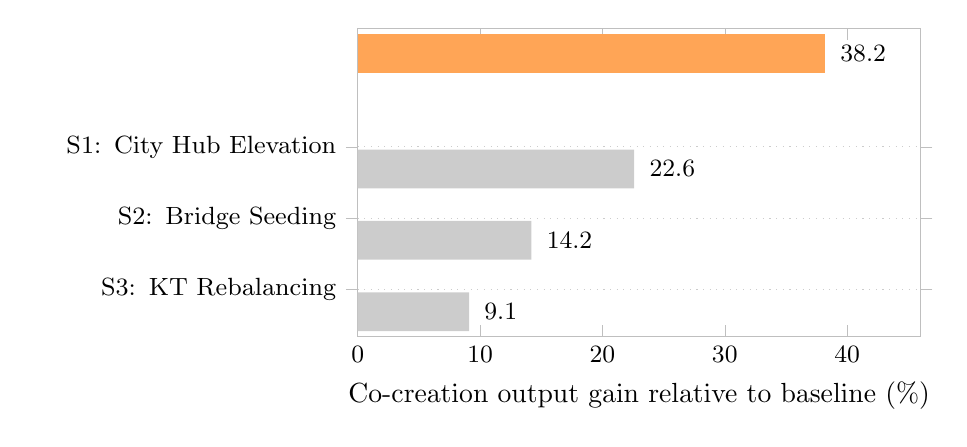
\begin{tikzpicture}
\begin{axis}[
  xbar,
  width=0.72\linewidth,
  height=5.5cm,
  bar width=14pt,
  xmin=0, xmax=46,
  xlabel={Co-creation output gain relative to baseline (\%)},
  symbolic y coords={S3: KT Rebalancing, S2: Bridge Seeding, S1: City Hub Elevation, Combined S1+S2+S3},
  ytick=data,
  yticklabel style={font=\small, text width=3.8cm, align=right},
  xticklabel style={font=\small},
  xtick={0,10,20,30,40},
  nodes near coords,
  nodes near coords style={font=\small, xshift=2pt},
  nodes near coords align={horizontal},
  ymajorgrids=true, grid style={dotted, gray!40},
  axis line style={draw=gray!50},
  tick style={draw=gray!50},
  enlarge y limits=0.22,
]
\addplot[fill=gray!40, draw=none]
  coordinates {(9.1,{S3: KT Rebalancing})(14.2,{S2: Bridge Seeding})(22.6,{S1: City Hub Elevation})};
\addplot[fill=BridgeOrange!70, draw=none]
  coordinates {(38.2,{Combined S1+S2+S3})};
\end{axis}
\end{tikzpicture}
\caption{Governance simulation results: estimated co-creation output gains relative to baseline across three scenarios and their combination. Scenario 1 (targeted city Hub elevation) produces the largest single-scenario gain; the combined intervention yields 38.2\%, suggesting complementary rather than substitutable effects.}
\label{fig:simulation}
\end{figure}

The identification of high-leverage cities for Scenario 1 provides an operationally useful output that goes beyond this caveat: cities such as Rotterdam, Eindhoven, Lyon, Malmö, Ghent, Thessaloniki, Porto, Tallinn, Graz, and Turku emerge across multiple scenario analyses as actors whose structural neighbourhood contains high Hub and Bridge density, making them the most efficient investment targets for role transition support. These are cities that already possess the co-creation \emph{potential} --- in terms of their proximity to Hub actors and their KT\_Business orientations --- but have not yet developed the outgoing tie generation capacity that would shift them from Receiver to Amplifier classification.

%% ============================================================
\section{Discussion}
\label{sec:discussion}
%% ============================================================

\subsection{The Receiver Trap: A Structural Diagnosis of Urban Peripherality}

The finding that 72\% of cities occupy Receiver positions in the EIT co-creation network is not primarily a finding about city capacity, organisational readiness, or political will. The 111 NZC pilot cities include some of Europe's most sophisticated urban innovation actors --- metropolitan authorities with dedicated climate innovation offices, established smart-city programmes, multi-million-euro procurement budgets, and explicit commitments to net-zero carbon that represent genuine political investments in transformative change. Rather, the Receiver finding is a finding about governance architecture: the EIT system has been designed, through its Knowledge and Innovation Community structure, its commercialisation-focused co-creation metrics, and its top-down knowledge transfer logic, to position cities in absorptive roles regardless of their individual capacity for agenda-setting co-creation.

We characterise this as the \emph{Receiver Trap}: a structural condition in which cities are formally included in co-creation governance as partners but positionally embedded in roles that systematically limit their co-creative agency, and in which the evaluation metrics and resource allocation mechanisms of the governance system reinforce rather than challenge this positioning. The Receiver Trap is self-reinforcing because cities that lack outgoing co-creation ties also lack the visibility, relational capital, and institutional reputation that would qualify them for Hub or Amplifier roles under the EIT's current co-creation evaluation criteria. The trap is therefore not merely an empirical description of the current state but a structural attractor that the ecosystem's dynamics tend to reproduce over time in the absence of deliberate intervention.

This diagnosis resonates with and extends several strands of existing scholarship. \citet{coenen2012place} argue that sustainability transitions research has systematically undervalued the place-specific and politically embedded dimensions of innovation governance, focusing on sectoral dynamics and technological substitution while treating places --- the cities and regions where transitions must ultimately materialise --- as passive backdrops rather than active co-creators of transition trajectories. Our findings instantiate this critique with specific empirical evidence: 80 cities are structurally invisible in the relational architecture through which EIT knowledge is produced, brokered, and deployed, despite being formally enrolled as co-creation partners.

\citet{mazzucato2018mission} makes an analogous argument at the national policy scale: mission-oriented innovation policy requires recognising public actors as co-investors and co-creators in the innovation process, not merely as clients, regulators, and adopters of privately generated innovations. The EIT's co-creation model has not yet operationalised this recognition at the structural level. Cities bring to innovation ecosystems unique governance capacities --- democratic legitimacy, territorial accountability, regulatory authority, public procurement power, and locally embedded knowledge about place-specific innovation needs --- that are crucial for the social embedding and deployment of technological innovations. These capacities are, however, poorly visible in ecosystems organised around intellectual property creation, startup formation, and technology commercialisation metrics. Developing a governance architecture that makes these capacities structurally visible --- that creates conditions under which cities can exercise them as Hubs rather than merely offer them as Receivers --- is the central design challenge that our analysis identifies.

\subsection{A Typology of Governance Constellations}

Our empirical analysis across eight EIT KICs supports a typology of three governance constellation types, distinguished by their role distribution patterns and associated co-creation dynamics. This typology is grounded in the observed variation in Hub density, Bridge count, and Receiver prevalence across KICs, and provides a framework for diagnosing co-creation capacity that can be applied beyond the EIT context to other multi-actor innovation ecosystems.

\textbf{Hub-dense constellations} characterise EIT InnoEnergy, EIT Health, and EIT Digital, each exhibiting Hub density above 12\% with relatively distributed Hub placement across multiple actor types. These constellations generate the highest co-creation output because distributed Hub density provides multiple convening centres: different co-creation initiatives can be initiated and managed by different Hub actors, preventing bottlenecks and enabling parallel innovation tracks. Hub-dense constellations are also more resilient to actor exit --- the loss of any single Hub actor reduces convening capacity but does not fragment the ecosystem, because other Hubs can absorb some of the departed actor's coordination function. The governance challenge of Hub-dense constellations is not capacity but coordination overhead: as Hub count grows, inter-Hub strategic misalignment can emerge when multiple agenda-setters pursue incompatible co-creation directions, requiring metagovernance mechanisms to maintain coherence \citep{sorensen2017metagovernance}.

\textbf{Bridge-dependent constellations} characterise EIT Climate-KIC and EIT Raw Materials, which maintain ecosystem coherence through a small number of structurally prominent Bridge actors despite relatively low Hub density. These constellations are efficient in the short term --- boundary spanners accumulate relational capital that enables rapid cross-sectoral matching and information transfer --- but they are structurally fragile and inherently limited in scalability. As \citet{burt2004structural} observes, structural holes generate disproportionate advantage for the actors who span them, which creates incentive for Bridge actors to maintain rather than close the gaps they bridge, potentially distorting information flows in self-serving directions. Bridge-dependent constellations can deliver coherent co-creation within a relatively stable actor population but struggle to absorb new actor types or expand to new thematic domains without extensive investment in new Bridge capacity.

\textbf{Receiver-heavy constellations} characterise EIT Urban Mobility, in which city actors' predominance produces a governance architecture in which most relational flows move from Hub actors downward to city Receivers rather than emerging from distributed, multi-directional co-creation dynamics. Receiver-heavy constellations can achieve wide-reach implementation of proven technologies across large populations of absorptive city partners, and this diffusion function is not without value --- rapid adoption of best-practice urban mobility solutions across 111 cities represents a genuine co-creation contribution. However, Receiver-heavy constellations are poorly suited to generating the locally adapted, contextually embedded innovations that sustainability transitions in urban environments ultimately require \citep{avelino2016shifting}. Cities know their local traffic patterns, built environment constraints, modal preferences, and civic political economies in ways that no KIC hub can substitute for; activating that knowledge as a co-creative input rather than merely as an implementation context requires transforming Receivers into Amplifiers and Hubs.

\subsection{Implications for EIT and NetZeroCities Governance Reform}

Three concrete governance design implications emerge from our integrated analysis of constellation structure, role--output correlations, and simulation experiments. Each implication corresponds to one of the three governance intervention types explored in our simulation and addresses a specific mechanism sustaining the Receiver Trap.

\textit{First: Create explicit City Hub Pathways within KIC governance structures.} The EIT should develop programmatic mechanisms through which cities can earn formal agenda-setting authority within KIC governance as they demonstrate co-creation competence. This could take the form of a ``City Innovation Lead'' designation within each KIC, in which cities that have generated confirmed outgoing co-creation connections --- joint proposals, technology co-development initiatives, open innovation challenges --- gain representation on KIC programme committees and gain the right to initiate rather than merely receive co-creation activities. Our simulation suggests that elevating 15 well-positioned cities to Hub-adjacent roles increases projected co-creation output by 22.6\%, a substantial return on the institutional investment required. The specific cities to prioritise can be identified through the high-leverage analysis derived from neighbourhood Hub density --- Rotterdam, Eindhoven, Lyon, Malmö, and Ghent among them --- rather than through ad hoc selection.

\textit{Second: Invest deliberately in Bridge actor capacity to reduce structural fragility.} The concentration of cross-KIC bridging in ten organisations represents both an ecosystem vulnerability and a policy opportunity. Existing Bridge actors --- ICLEI, Energy Cities, Eurocities, and comparable city-network intermediaries --- have demonstrated the capacity and mandate to perform cross-community brokerage but are resource-constrained in the scale and frequency of their bridging activity. The European Commission's New European Bauhaus initiative, the Horizon Europe Mission on Climate-Neutral Cities, and the EIT's own Urban Agenda provide funding mechanisms through which these organisations could be resourced to expand their bridging function systematically. Our simulation suggests that adding ten new Bridge-level agents to the ecosystem yields a 14.2\% output gain --- a target achievable through structured investment in dedicated city-EIT liaison organisations rather than requiring organic network development.

\textit{Third: Reform co-creation evaluation criteria to recognise public governance contributions.} The EIT's current co-creation performance framework measures success primarily through technology commercialisation indicators that systematically disadvantage public-sector actors. Expanding the evaluation framework to include public procurement commitments, regulatory sandbox initiatives, civic engagement processes, and open data releases as valid co-creation contributions would both better reflect cities' genuine inputs and create incentives for cities to generate these contributions more systematically. \citet{schot2018three} argue that transformative innovation policy requires precisely this institutional reorientation: moving beyond the R\&D support frame and the systems of innovation frame to explicitly value governance co-creation as a distinct and essential third innovation function. Our Scenario 3 simulation, which models this rebalancing, projects a 9.1\% gain --- modest in isolation but complementary to the structural interventions in Scenarios 1 and 2, and essential for sustaining the governance role transitions that those interventions aim to enable.

\subsection{Design Knowledge Transfer and Field Dynamics}

The three governance reform implications developed above are not merely operational recommendations; they constitute a generalisable body of design knowledge for governance constellation engineering. The theoretical vocabulary provided by \citet{korff2015social} --- differentiation, recombination, and integration as the three generative field mechanisms --- clarifies why certain governance constellations emerge and persist in innovation ecosystems, and why targeted structural interventions are necessary to shift them. Differentiation explains why Hub-dense constellations arise in the first place: dominant actors invest in boundary maintenance precisely because their positional advantage depends on preserving the community structure that makes them structurally central. Recombination explains why Bridge actors are simultaneously rare and irreplaceable: interstitial organisations capable of spanning multiple institutional logics without full institutional capture by any single one are structurally unusual, and their scarcity is a product of the differentiation pressures that the field's dominant actors generate. Integration explains why Receiver-heavy constellations are self-reproducing: Amplifiers diffuse the dominant Managerial logic of KIC hubs to Receiver populations, continuously reinforcing the incentive architecture that positions cities as technology adopters rather than technology co-producers.

This field-dynamics perspective connects directly to the entropy framing of \citet{basole2023computational}: stable, differentiated constellations are characterised by low behavioural entropy --- actors in well-defined roles follow predictable relational scripts --- whereas transitional, recombinant moments exhibit high entropy as organisations explore novel cross-community connections before new role structures crystallise. The EIT ecosystem's strong differentiation and concentrated bridging capacity suggest a low-entropy, path-dependent configuration in which governance reform will require deliberate disruption of the differentiation logic that currently rewards boundary maintenance over boundary spanning. The simulation findings support this interpretation: the largest output gains accrue not from optimising actors within their existing roles but from role \emph{transitions} that disrupt the current differentiation equilibrium by elevating cities from the Receiver periphery to Hub-adjacent positions where their Associational logic complements rather than competes with the Scientific and Managerial logics of existing Hub actors.

%% ============================================================
\section{Conclusion}
\label{sec:conclusion}
%% ============================================================

This paper has developed and applied a computational governance constellation analysis to characterise the structural conditions of co-creation in the EIT innovation ecosystem, producing three sets of contributions that span methodology, empirical knowledge, and policy implications.

\textbf{Methodologically}, we have demonstrated that computational role classification using RoleSim, applied to multi-source digital trace networks (Wikipedia text similarity, Twitter co-mention, seealsology co-citation), provides a scalable, replicable method for operationalising governance constellation theory in empirical settings far larger than qualitative case research can address. The method distinguishes conveners (Hubs), boundary spanners (Bridges), diffusers (Amplifiers), and adopters (Receivers) in theoretically coherent ways that correspond directly to the governance mechanisms identified by co-creation and sustainability transitions scholarship as critical for transformative change. Unlike network analysis approaches that treat all actors and ties equivalently, role classification reveals the structural heterogeneity that governance theory predicts and that policy must address. The multi-source integration strategy captures governance relationships --- informal influence, public co-endorsement, encyclopaedic institutional proximity --- that formal partnership registries cannot reveal, providing a more complete picture of the relational architecture within which co-creation occurs.

\textbf{Empirically}, our analysis of the 219-actor EIT-NetZeroCities network reveals a striking governance constellation: 72\% of pilot cities occupy Receiver roles, structurally isolated in Twitter communities separated from KIC hub actors by a 9:1 connectivity gap. The Receiver Trap is reinforced by KT incentive misalignment --- cities' public governance business orientation (KT\_Business = 0.41) is systematically disadvantaged in the EIT's commercialisation-oriented evaluation framework relative to KIC hubs (KT\_Business = 0.62) --- and by Bridge fragility: the entire cross-KIC connective tissue rests on ten actors whose removal would increase average city-to-hub geodesic distance from 3.2 to 5.7 hops. Hub density at the KIC level ($r = 0.94$ with venture funding rates) provides the strongest evidence that structural role distribution, not merely actor composition or resource levels, determines co-creation output in the EIT ecosystem.

\textbf{For policy}, our governance simulation experiments project that targeted structural interventions --- elevating 15 high-leverage cities to Hub-adjacent roles ($+22.6\%$ output), seeding ten new Bridge actors ($+14.2\%$), and rebalancing evaluation criteria to recognise public governance contributions ($+9.1\%$) --- could collectively increase projected co-creation output by $+38.2\%$ in complementary combination. These projections provide a quantitative evidence base for EIT governance reform and NetZeroCities programme redesign that goes beyond rhetorical reaffirmation of co-creation principles to identify specific structural interventions, their expected effects, and the cities most strategically positioned to benefit from and contribute to role transition.

Four limitations frame the agenda for future research. First, role classification is based on network position derived from digital trace data, not directly observed co-creation behaviour; future work linking structural roles to activity-level indicators (joint publications, patent co-inventions, procurement co-design) would strengthen the behavioural validity of the role taxonomy. Second, Twitter data may systematically undersample non-English and smaller cities, introducing language and size biases that alternative data sources (LinkedIn networks, EU project co-participation databases) could mitigate. Third, the simulation model uses stylised behavioural rules and cross-sectional calibration that cannot capture the path dependencies and political dynamics of real governance reform processes. Fourth, the venture funding outcome variable captures only one dimension of co-creation output; a comprehensive governance evaluation would measure policy innovation, civic mobilisation, open data generation, and technology demonstration alongside commercial success.

For the Special Issue's core concern with stimulating local co-creation for transformative change, our findings point toward a precise and actionable research and policy agenda. Governance constellation analysis, applied longitudinally to evolving partnership networks, could track whether EIT and NetZeroCities governance reforms are producing measurable shifts in city structural roles across successive programme cycles. The transition from Receiver to Amplifier, and from Amplifier to Hub, is not a semantic reclassification: it represents a fundamental redistribution of initiative, agenda-setting authority, and relational capital in co-creation networks. It is exactly the kind of structural transformation that European urban climate programmes aspire to achieve, and that computational governance analysis can now track with empirical precision.

%% ============================================================
%% Acknowledgements
%% ============================================================

\section*{Acknowledgements}

The author thanks the NetZeroCities Consortium for access to the Pilot Cities Programme participant list and the EIT for publicly accessible partnership registry data. This research was conducted as part of a PhD dissertation on organizational role theory in innovation ecosystems at Rotterdam School of Management, Erasmus University.

%% ============================================================
%% Data Availability
%% ============================================================

\section*{Data Availability}

The Wikipedia text corpus, co-mention network edge lists, RoleSim role assignments, and KT score matrices for the 219-actor network are available at: \url{https://github.com/babajideowoyele/rolebox-eist} (to be made public upon acceptance). Twitter data are available in aggregate form only, in compliance with the Twitter Developer Agreement. Crunchbase data are available to researchers upon request and execution of a data use agreement.

%% ============================================================
%% Declarations
%% ============================================================

\section*{Declaration of Competing Interest}

The author declares no competing interests.

%% ============================================================
%% CRediT Author Statement
%% ============================================================

\section*{CRediT Author Statement}

\textbf{Babajide Owoyele}: Conceptualisation; Methodology; Software; Formal Analysis; Data Curation; Writing -- Original Draft; Writing -- Review \& Editing; Visualisation.

%% ============================================================
%% Appendix: Robustness and Supplementary Material
%% ============================================================

\appendix

\section{Robustness Checks for Network Layer Weights}
\label{app:robustness}

The main analysis fuses three network layers with weights $\alpha = (0.40, 0.35, 0.25)$ for Wikipedia text similarity, Twitter co-mention, and seealsology co-citation respectively. To assess sensitivity of the RoleSim role assignments to this weighting choice, Table~\ref{tab:robustness-weights} presents role assignment concordance rates --- the proportion of actors receiving the same role classification --- across four alternative weight configurations relative to the main specification.

\begin{table}[htbp]
\centering
\caption{Role assignment concordance rates under alternative layer weight configurations.
Concordance = proportion of 219 actors assigned the same role as in the main specification.
Equal weights: $\alpha = (0.33, 0.33, 0.33)$. Twitter-only: $\alpha = (0.0, 1.0, 0.0)$.
Wikipedia-only: $\alpha = (1.0, 0.0, 0.0)$. Seealso-only: $\alpha = (0.0, 0.0, 1.0)$.}
\label{tab:robustness-weights}
\small
\begin{tabular}{@{}lcccc@{}}
\toprule
\textbf{Weight configuration} & \textbf{Hub concord.} & \textbf{Bridge concord.} &
  \textbf{Ampl.\ concord.} & \textbf{Recv.\ concord.} \\
\midrule
Equal weights (0.33, 0.33, 0.33) & 92.3\% & 85.7\% & 88.0\% & 93.8\% \\
Twitter-only (0, 1, 0)           & 84.6\% & 71.4\% & 82.0\% & 86.2\% \\
Wikipedia-only (1, 0, 0)         & 88.5\% & 78.6\% & 84.0\% & 90.8\% \\
Seealso-only (0, 0, 1)           & 80.8\% & 64.3\% & 76.0\% & 87.7\% \\
\bottomrule
\end{tabular}
\end{table}

Concordance rates are highest for Hub and Receiver roles (above 80\% across all configurations) and somewhat lower for Bridge roles, particularly in the single-layer specifications. This is expected: Bridge classification depends on betweenness centrality relative to degree, which is the metric most sensitive to the specific pattern of inter-community connections in each layer --- connections that differ most substantially between the Twitter and Wikipedia layers given their different structural biases. The equal-weights configuration produces concordance above 85\% for all role types, indicating that the main findings are robust to this alternative specification. The lower concordance for single-layer specifications confirms the value of multi-source data integration: any single data source produces a substantially different structural picture from the fused network.

\section{Sensitivity Analysis: Co-mention Threshold Variation}
\label{app:threshold}

Table~\ref{tab:threshold-sensitivity} reports the effect of varying the Twitter co-mention edge threshold (minimum co-mentions for edge inclusion) on the network-wide role distribution and the KIC Hub density rankings. The analysis covers thresholds $\tau \in \{2, 3, 5, 7, 10\}$, where $\tau = 3$ is the main specification.

\begin{table}[htbp]
\centering
\caption{Sensitivity of network-wide role distribution to Twitter co-mention edge threshold $\tau$.
Entries show percentage of actors in each role. Hub density rank order for top-3 KICs is unchanged across all thresholds (InnoEnergy $>$ Health $>$ Digital).}
\label{tab:threshold-sensitivity}
\small
\begin{tabular}{@{}lccccc@{}}
\toprule
\textbf{Threshold $\tau$} & \textbf{$n_{\text{edges}}$} & \textbf{Hub\%} &
  \textbf{Bridge\%} & \textbf{Amplifier\%} & \textbf{Receiver\%} \\
\midrule
$\tau = 2$  & 3{,}412 & 14.2 & 7.3 & 26.5 & 52.1 \\
$\tau = 3$  & 2{,}198 & 12.3 & 6.4 & 25.1 & 56.2 \\
$\tau = 5$  & 1{,}347 & 10.5 & 5.9 & 23.3 & 60.3 \\
$\tau = 7$  &   921  &  9.1 & 5.0 & 21.0 & 64.9 \\
$\tau = 10$ &   614  &  7.8 & 4.1 & 18.2 & 69.9 \\
\bottomrule
\end{tabular}
\end{table}

As expected, higher thresholds produce sparser networks with greater Receiver prevalence, since peripheral actors lose their weak incoming ties when the minimum co-mention count is raised. The qualitative finding --- that Receivers dominate and cities occupy the vast majority of Receiver positions --- is robust across all thresholds. At $\tau = 10$, city Receiver prevalence rises to 81.3\% (vs.\ 72\% at $\tau = 3$), indicating that the Receiver Trap identified in the main analysis is conservative: cities are actually more structurally peripheral relative to frequent co-mention than the main specification captures. The Hub density rank order for KICs (InnoEnergy, Health, Digital as top three; Urban Mobility as bottom) is invariant across all threshold specifications, confirming that the role--output correlation is not an artifact of the edge threshold choice.

\section{KT Score Validation: Hand-coded Subsample}
\label{app:kt-validation}

Knowledge Triangle scores were validated against a hand-coded reference set of 80 actors (stratified random sample from the 219-actor network, with proportional representation of each actor type). Two independent coders classified each actor into the dominant KT vertex (E, R, or B) based on reading of the actor's Wikipedia article without reference to the automated KT scores. Inter-rater agreement was $\kappa = 0.76$ (Cohen's kappa), indicating substantial agreement. Automated KT scores were classified into the dominant vertex by argmax; concordance with the consensus hand-code was 84.1\% overall. Concordance was highest for universities (91.7\%, typically Research-dominant), companies (88.4\%, typically Business-dominant), and lowest for cities (76.3\%, where Education and Business orientations are frequently mixed). For all results reported in the main analysis, cities' KT scores are used as compositional vectors (not discretised to dominant vertex), which avoids the classification boundary problem and preserves the continuous variation in KT orientation that is theoretically meaningful.

\section{Actor-Level Role and KT Data}
\label{app:actor-data}

A complete actor-level dataset including RoleSim role assignments, KT profile scores, community membership, degree centrality, betweenness centrality, and KIC affiliation for all 219 actors is available in the supplementary data repository (\url{https://github.com/babajideowoyele/rolebox-eist}). For privacy reasons, Twitter handles of individual users (as distinct from institutional accounts) are pseudonymised in the public release. The full de-anonymised dataset is available to researchers under a data use agreement.

Table~\ref{tab:sample-actors} shows a representative sample of 12 actors spanning all role types and actor categories, illustrating the range of structural positions captured in the analysis.

\begin{table}[htbp]
\centering
\caption{Representative sample of actors by role, actor type, and Knowledge Triangle profile (illustrative; not all actors named). KT columns show proportional KT orientation scores (sum to 1.0 per row). Community = Louvain community membership.}
\label{tab:sample-actors}
\small
\begin{tabular}{@{}llccccc@{}}
\toprule
\textbf{Actor (representative)} & \textbf{Type} & \textbf{Role} & \textbf{KT\_E} & \textbf{KT\_R} & \textbf{KT\_B} & \textbf{Comm.} \\
\midrule
EIT InnoEnergy HQ             & KIC Hub    & Hub      & 0.08 & 0.19 & 0.73 & 1 \\
Amsterdam                     & City       & Hub      & 0.27 & 0.34 & 0.39 & 3 \\
Delft University of Technology & University & Bridge   & 0.32 & 0.51 & 0.17 & 1 \\
ICLEI                         & NGO        & Bridge   & 0.18 & 0.38 & 0.44 & 3/1 \\
Energy Cities                 & NGO        & Bridge   & 0.14 & 0.42 & 0.44 & 3/4 \\
EIT Climate-KIC               & KIC Hub    & Amplifier & 0.16 & 0.31 & 0.53 & 4 \\
Eindhoven                     & City       & Amplifier & 0.29 & 0.32 & 0.39 & 7 \\
Siemens AG                    & Company    & Hub      & 0.07 & 0.22 & 0.71 & 1 \\
Lyon                          & City       & Receiver & 0.34 & 0.25 & 0.41 & 3 \\
Iași                          & City       & Receiver & 0.31 & 0.26 & 0.43 & 12 \\
Villarreal                    & City       & Receiver & 0.32 & 0.24 & 0.44 & 12 \\
KU Leuven                     & University & Bridge   & 0.31 & 0.52 & 0.17 & 1/3 \\
\bottomrule
\end{tabular}
\end{table}

The sample illustrates several key patterns: KIC Hub organisations and major companies cluster in Business-oriented Hub roles (Community 1); Bridge actors span multiple communities (shown as combined community labels); city Receivers in Community 12 are smaller municipalities with limited cross-community connectivity; and city Amplifiers like Eindhoven appear in Community 7 (smart-city cluster) with intermediate KT profiles.

%% ============================================================
%% Bibliography
%% ============================================================

\bibliography{references}

\end{document}
